% **************************************************
% Document Class Definition
% **************************************************
\documentclass[%
    paper=A4,               % paper size --> A4 is default in Germany
    onside,                 % onesite or twoside printing
    parskip=half,           % spacing value / method for paragraphs
    chapterprefix=true,     % prefix for chapter marks
    11pt,                   % font size
    headings=normal,        % size of headings
    bibliography=totoc,     % include bib in toc
    listof=totoc,           % include listof entries in toc
    titlepage=on,           % own page for each title page
    captions=tableabove,    % display table captions above the float env
    chapterprefix=false,    % do not display a prefix for chapters
    appendixprefix=false,    % but display a prefix for appendix chapter
    draft=false,            % value for draft version
]{scrreprt}%


% **************************************************
% Setup YOUR thesis document in this file !
% **************************************************
% !TEX root = thesis.tex


% **************************************************
% Files' Character Encoding
% **************************************************
\PassOptionsToPackage{utf8}{inputenc}
\usepackage{inputenc}


% **************************************************
% Information and Commands for Reuse
% **************************************************
\newcommand{\thesisTitle}{A Practical Analysis of UEFI Threats Against Windows~11}
\newcommand{\thesisName}{Joshua Machauer}
\newcommand{\thesisSubject}{Bachelor's Thesis}
\newcommand{\thesisDate}{December 25, 2022}
\newcommand{\thesisDateGerman}{25. Dezember 2022}
\newcommand{\thesisVersion}{Draft 1.0}

\newcommand{\thesisFirstReviewer}{Prof. Dr. Jean-Pierre Seifert}
\newcommand{\thesisFirstReviewerUniversity}{\protect{Technische Universität Berlin}}
\newcommand{\thesisFirstReviewerDepartment}{Electrical Engineering and Computer Science}

\newcommand{\thesisSecondReviewer}{Prof. Dr. Stefan Schmid}
\newcommand{\thesisSecondReviewerUniversity}{\protect{Technische Universität Berlin}}
\newcommand{\thesisSecondReviewerDepartment}{Electrical Engineering and Computer Science}

\newcommand{\thesisFirstSupervisor}{Hans Niklas Jacob}
\newcommand{\thesisSecondSupervisor}{Christian Werling}

\newcommand{\thesisUniversity}{\protect{Technische Universität Berlin}}
\newcommand{\thesisUniversityDepartment}{Electrical Engineering and Computer Science}
\newcommand{\thesisUniversityInstitute}{Institute of Software Engineering and Theoretical Computer Science}
\newcommand{\thesisUniversityGroup}{Security in Telecommunications (SecT)}
\newcommand{\thesisUniversityCity}{Berlin}
\newcommand{\thesisUniversityStreetAddress}{Ernst-Reuter-Platz 7}
\newcommand{\thesisUniversityPostalCode}{10587}



% **************************************************
% Debug LaTeX Information
% **************************************************
%\listfiles


% **************************************************
% Load and Configure Packages
% **************************************************
\usepackage[english]{babel} % babel system, adjust the language of the content
\usepackage{acronym}[printonlyused]
\PassOptionsToPackage{% setup clean thesis style
    figuresep=colon,%
    hangfigurecaption=false,%
    hangsection=true,%
    hangsubsection=true,%
    sansserif=false,%
    configurelistings=true,%
    colorize=full,%
    colortheme=bluemagenta,%
    configurebiblatex=true,%
    bibsys=biber,%
    bibfile=bib-refs,%
    %bibstyle=alphabetic,%			-> citations with alphabetic enumeration
    %bibstyle=numeric-comp,%		-> citations with numeric compressed numeric sorting
    bibstyle=ieee-alphabetic,%		-> citations with IEEE transactions-like style with numeric labels
    %bibsorting=nty,% 
    bibsorting=none,%				-> sorted in the order of the citations from start to finish
}{cleanthesis}
\usepackage{cleanthesis}

\hypersetup{% setup the hyperref-package options
    pdftitle={\thesisTitle},    %   - title (PDF meta)
    pdfsubject={\thesisSubject},%   - subject (PDF meta)
    pdfauthor={\thesisName},    %   - author (PDF meta)
    plainpages=false,           %   -
    colorlinks=false,           %   - colorize links?
    pdfborder={0 0 0},          %   -
    breaklinks=true,            %   - allow line break inside links
    bookmarksnumbered=true,     %
    bookmarksopen=true          %
}


\graphicspath{{./images/}{./figures/}}
\usepackage{svg}

\usepackage{multirow}
\usepackage[shortcuts]{extdash}

\usepackage{textcmds}



% **************************************************
% Document CONTENT
% **************************************************
\begin{document}

% uncomment the following command to fill up pages with
% whitespace instead of aligning the first and last lines
% of a page (see \raggedbottom vs. \flushbottom)
%\raggedbottom

% --------------------------
% rename document parts
% --------------------------
\renewcaptionname{english}{\figurename}{Fig.}
\renewcaptionname{english}{\tablename}{Tab.}

% --------------------------
% Front matter
% --------------------------
\pagenumbering{roman}			% roman page numbing (invisible for empty page style)
\pagestyle{empty}				% no header or footers
% !TEX root = ../thesis.tex
%
% ------------------------------------  --> cover title page
\begin{titlepage}
	\pdfbookmark[0]{Cover}{Cover}
	\flushright
	\hfill
	\vfill
	{\LARGE\thesisTitle \par}
	\rule[5pt]{\textwidth}{.4pt} \par
	{\Large\thesisName}
	\vfill
	\textit{\large\thesisDate} \\
	Version: \thesisVersion
\end{titlepage}


% ------------------------------------  --> main title page
\begin{titlepage}
	\pdfbookmark[0]{Titlepage}{Titlepage}
	\tgherosfont
	\centering

	{\Large \thesisUniversity} \\[4mm]
	
\includegraphics[width=6cm]{gfx/Clean-Thesis-Logo} \\[2mm]
	\textsf{\thesisUniversityDepartment} \\
	\textsf{\thesisUniversityInstitute} \\
	\textsf{\thesisUniversityGroup} \\

	\vfill
	{\large \thesisSubject} \\[5mm]
	{\LARGE \color{ctcolortitle}\textbf{\thesisTitle} \\[10mm]}
	{\Large \thesisName} \\

	\vfill
	\begin{minipage}[t]{.27\textwidth}
		\raggedleft
		\textit{1. Reviewer}
	\end{minipage}
	\hspace*{15pt}
	\begin{minipage}[t]{.65\textwidth}
		{\Large \thesisFirstReviewer} \\
		{\small \thesisFirstReviewerDepartment} \\[-1mm]
		{\small \thesisFirstReviewerUniversity}
	\end{minipage} \\[5mm]
	\begin{minipage}[t]{.27\textwidth}
		\raggedleft
		\textit{2. Reviewer}
	\end{minipage}
	\hspace*{15pt}
	\begin{minipage}[t]{.65\textwidth}
		{\Large \thesisSecondReviewer} \\
		{\small \thesisSecondReviewerDepartment} \\[-1mm]
		{\small \thesisSecondReviewerUniversity}
	\end{minipage} \\[10mm]
	\begin{minipage}[t]{.27\textwidth}
		\raggedleft
		\textit{Supervisors}
	\end{minipage}
	\hspace*{15pt}
	\begin{minipage}[t]{.65\textwidth}
		\thesisFirstSupervisor\ and \thesisSecondSupervisor
	\end{minipage} \\[10mm]

	\thesisDate \\

\end{titlepage}


% ------------------------------------  --> lower title back for single page layout
\hfill
\vfill
{
	\small
	\textbf{\thesisName} \\
	\textit{\thesisTitle} \\
	\thesisSubject, \thesisDate \\
	Reviewers: \thesisFirstReviewer\ and \thesisSecondReviewer \\
	Supervisors: \thesisFirstSupervisor\ and \thesisSecondSupervisor \\[1.5em]
	\textbf{\thesisUniversity} \\
	\textit{\thesisUniversityGroup} \\
	\thesisUniversityInstitute \\
	\thesisUniversityDepartment \\
	\thesisUniversityStreetAddress \\
	\thesisUniversityPostalCode\ \thesisUniversityCity
}
		% INCLUDE: all titlepages
\cleardoublepage

% !TEX root = ../thesis.tex
%
%************************************************
% Declaration
%************************************************
\pdfbookmark[0]{Selbst\"andigkeitserkl\"arung}{Selbst\"andigkeitserkl\"arung}
\chapter*{Selbst\"andigkeitserkl\"arung}
\label{sec:declaration}
\thispagestyle{empty}

Hiermit erkl\"are ich, dass ich die vorliegende Arbeit selbstst\"andig und eigenh\"andig sowie ohne
unerlaubte fremde Hilfe und ausschlie\ss{}lich unter Verwendung der aufgef\"uhrten Quellen und
Hilfsmittel angefertigt habe.

\bigskip

\noindent\textit{\thesisUniversityCity, den \thesisDateGerman}

\smallskip

\begin{flushright}
	\begin{minipage}{5cm}
		\rule{\textwidth}{1pt}
		\centering\thesisName
	\end{minipage}
\end{flushright}

%*****************************************
%*****************************************
\cleardoublepage

\pagestyle{plain}				% display just page numbers
% !TEX root = ../thesis.tex

% http://williamstallings.com/Extras/Abstract.html
% https://www.enago.com/academy/abstract-versus-introduction-difference/

\pdfbookmark[0]{Abstract}{Abstract}
\addchap*{Abstract}
\label{sec:abstract}

% motivation
In Computer Security one of the most feared security threats is a rootkit, executing at the beginning of a computers boot chain, before the operating system and accompanying antivirus programs. With the widespread adaption of standardized UEFI firmware these threats have become less machine dependent and can now target a host of systems at once.
% problem statement
Past analyses about bootkits have been case studies of their appearances in the wild, this thesis instead aims to be a more practical approach by developing a bootkit and analyzing the challenges doing so.
% approach
We restrict our analysis by assuming an attacker has already gained read and write access to the BIOS image and is thus only facing security mechanisms involved during and with execution of the bootkit.
% results
Our bootkit was able to achieve elevated execution on Windows 11 by exploiting unrestricted hard drive access to edit Windows Registries, this was also possible on BitLocker encrypted hard drives by keylogging the Recovery Key.
% conclusions
UEFI makes it very easy for an attacker who has gained access to the System Firmware to leverage its powers and gain full control over the system.

\vspace*{20mm}

{\usekomafont{chapter}Abstract (different language)}
\label{sec:abstract-diff}

\blindtext
		% INCLUDE: the abstracts (english and german)
\cleardoublepage
%
% !TeX root = ../thesis.tex
%
\pdfbookmark[0]{Acknowledgement}{Acknowledgement}
\chapter*{Acknowledgement}
\label{sec:acknowledgement}
\thispagestyle{empty}


 % INCLUDE: acknowledgement
\cleardoublepage
%
\currentpdfbookmark{\contentsname}{toc}
\setcounter{secnumdepth}{3}
\setcounter{tocdepth}{3}		% define depth of toc
\tableofcontents				% display table of contents
\cleardoublepage

% --------------------------
% Body matter
% --------------------------
\pagenumbering{arabic}			% arabic page numbering
\setcounter{page}{1}			% set page counter
\pagestyle{scrheadings}			% header and footer style

%\part{Example Part}
% !TeX root = ../thesis.tex

% https://www.enago.com/academy/abstract-versus-introduction-difference/
% https://www.student.unsw.edu.au/introductions
% https://www.scribbr.com/dissertation/introduction-structure/

\chapter{Introduction}


% what is UEFI
As the first piece of software that is run on your computer, UEFI holds an immense amount of responsibility during system initialization, attacks targeting your operating system from this environment are executed long before

what does it different than bios
this helps write platform independent code
uefi threats:
% definition of rootkit and bootkit
A rootkit is a collection of software designed to grant a threat actor control over a system, typically with malicious intend.
Rootkits set up a backdoor exploit and may deliver additional malware while leveraging their privileges to remain hidden.
There are different types of rootkits such as User Mode, Kernel Mode, Bootkits (bootloader rootkits), Hypervisor and Firmware rootkits.
\cite{crowdstrike, techtarget}
\TODO{consult abstract for similar definition, how easy uefi makes it to write hardware independent payload}
Firmware rootkits targets the software running during the boot process, which is responsible for the system initialization. This is done before the operating system is executed making them particularly hard to find, they are also persistent across operating system installation or hard drive replacements.
\cite{crowdstrike}


look at UEFI + threats against windows
danger of uefi infection
in recent years root and bootkits have popped up in the wild and been analysed
differences of root-/bootkits
reason about infection scenarios
we will discuss their commonalities
attack vectors:
- storage based
- memory based
implement a storage based ourselves
analyse security mechanism to prevent these attacks by attempting an attack itself
discuss security mechanisms we encounter
increasing security mechanisms
reflect their weaknesses
how to potentially evade them
- analyse countermeasures against UEFI threats
- Trusted Boot: KMCI from windows
- Secure Boot
- TPM
- Bitlocker
- firmware lock + signed capsule update
-



We start off introducing all background information necessary to understand this thesis in Chapter 2. With this knowledge we then look at analyses of previously discovered UEFI threats in Chapter 3. In Chapter 4 we start our practical approach by implementing a UEFI attack of our own to analyse security mechanism faced when attempting attacks from the UEFI environment. Afterwards we dicuss the impact of our findings as well as potential mitigation techniques in Chapter 5. Chapter 6 concludes ...

% !TeX root = ../../thesis.tex

\chapter{\acs{UEFI}/\acs{PI}}

\textcquote{uefi-spec-overview}{The \ac{UEFI} specifications define a new model for the interface between personal-computer \ac{OS} and \ac{PF}. \textelp{} Together, these provide a standard environment for booting an \ac{OS} and running pre-boot applications}.
The specifications making up this model are:

\begin{itemize}
    \item \acs{ACPI} Specification
    \item \acs{UEFI} Specification
    \item \acs{UEFI} Shell Specification
    \item \acs{UEFI} \acs{PI} Specification
    \item \acs{UEFI} \acs{PI} Distribution Packaging Specification
    \item \acs{TCG} \acs{EFI} Platform Specification
    \item \acs{TCG} \acs{EFI} Protocol Specification
\end{itemize}

The \ac{ACPI} and \ac{UEFI} \ac{PI} Distribution Packaging Specification are not required to be able to follow this thesis.
As for the other specifications, we briefly summarize the relevant content.


\clearpage
% !TeX root = ../../thesis.tex

\section{\acf{UEFI}}

The \ac{UEFI} specification is a pure interface specification, describing a programmatic interface for boot applications to interact with the \ac{PF}.
It states what interfaces, structures and abstractions a \ac{PF} has to offer and implement and what an boot applications such as \ac{OS} loaders may use \cite{beyond-bios}.

It was designed to replace the legacy \acl{BF} \ac{BIOS}, while also providing backwards compatibility with a \acf{CSM} allowing \ac{UEFI} firmware to boot legacy \ac{BIOS} applications \cite{beyond-bios}.
It is aimed to be a complete solution, abstracting all platform features and capabilities in a way so that boot loaders require no knowledge about the underlying hardware \cite[1.3]{uefi-spec}.

The \ac{UEFI} interfaces are defined in the \code{C} programming language.
During boot system resources are owned and managed by the \ac{UEFI} firmware until the \ac{OS} explicitly assumes control over the system.
On \code{x64} \ac{CPU} architecture the \ac{PF} hands over execution in \code{64-bit} long mode which includes memory protection.
Paging is also enabled and the virtual memory is identify mapped, meaning virtual addresses equal physical addresses, while most regions are read, write and execute.
The \ac{CPU} is in uniprocessor mode and a sufficent amount of stack is available \cite[Section 2.3.4]{uefi-spec}.

\subsection{\acf{GUID}}

The \ac{UEFI} environment depends on \acp{GUID}, also known \acp{UUID} to uniquely identify a variety of things, such as protocols, files, hard drive paritions.
\acp{GUID} are 128-bit long, statistically unique identifiers and can be generated on demand and without a centralized authority, statistically guaranteeing that there will be no duplicates on a system that combines hard and software from multiple vendors \cite{rfc-4122}.

\subsection{\acf{GPT}}

Partitions allow a disk to be distinctly separated into logical disks, allowing for each to be formatted with a different file systems.
Prior to \ac{UEFI} disks have been paritioned using the \ac{MBR} parition table, supporting up to 4 different partitions.
The \ac{MBR} is stored within the first sector, also optionally containing 424 bytes of bootable code through which the \ac{BIOS} boots \cite[Section 13.3.1]{uefi-spec}.
\ac{UEFI} is still backwards compatible with \ac{MBR} partitioned disks and contained on each disk, but \ac{UEFI} does not execute the boot code.
The \ac{MBR} is used in two different ways by the \ac{UEFI} environment, either as a legacy \ac{MBR} or a protective \ac{MBR}.
With the legacy \ac{MBR}, \ac{UEFI} uses the partitions defined in the \ac{MBR} parition table, where as the protective \ac{MBR} only has one partition spanning the entire disk.
The protective partition is for legacy devices and in reality \ac{GPT} partitioning is used to separate the disk.
For this \ac{UEFI} defines two \ac{OS} types used in \ac{MBR} parition entries.
One identifies the \ac{ESP}, the parition \ac{UEFI} boots from, within the legacy \ac{MBR} partition table and the other indicates that a protective parition is used \cite[Section 5]{uefi-spec}.
\cite[Section 5]{uefi-spec} defines the \ac{GPT} disk layout, with the \ac{GPT} format \ac{LBA} are 64 bit instead of 32 bit, allowing to support drives with up to 9400000000 \ac{TB} of storage, where as \ac{MBR} is limited to 2 \ac{TB}.
This is accompanied by allowing many more than 4 partitions, with Windows supporting up to 128 \cite{microsoft-windows-and-gpt-faq}.
\ac{GUID} are used to identify paritions and parition types, but also offering a human readable parition name.
\ac{GPT} also has a primary and a backup parition table for redundancy pruposes, the primary table follows the \ac{MBR} sector and the backup is at the end of the disk.

\subsection{\acf{ESP}}

The \ac{ESP} can reside any media that is supported by the \ac{UEFI} firmware and has to be \ac{FAT}32 formatted \cite[Section 13.3]{uefi-spec}.
It must contain an \lstinline{EFI} root directory \cite[Section 13.3.1.3]{uefi-spec} and all \ac{UEFI} applications, that are to be launched directly by the \ac{UEFI} firmware have to be located in subdirectories below the \lstinline{EFI} driectory \cite[Section 13.3.1.3]{uefi-spec}. Drivers and indirectly loaded applcations have no storage restrictions. Vendors are to use vendor\-/specifically named subdirectories within the \lstinline{EFI} directory. Fixed disks have no restrictions on the amount of \acp{ESP} present, whereas removable media is only allowed to have one \ac{ESP}, so that boot behavior is deterministic. In general the \ac{ESP} is identified by a specific \ac{GUID}, but implementations are allowed to support accordingly structured \ac{FAT} partitions. Since there is no limitation on the amount of \acp{ESP}, boot applications can share the drive with their \ac{OS}, or can be accumulated in a single system\-/wide \ac{ESP} \cite[Section 13.3.3]{uefi-spec}.


\subsection{\acs{UEFI} Images}

\ac{UEFI} Images are files containting executable code, they use a subset of the \ac{PE32}+ file format with a modified header signature.
The format comes with relocation tables, making it possible for the images to be executed in place or to be loaded at non pre\-/determined memory addresses.
They support multiple CPU architectures such as IA, ARM, RISC-V and x86.
There are three different subtypes of executables: applications, boot and runtime drivers. They mainly differ by their memory type and how it behaves.
Loading and transferring execution are two separate steps, so that security policies can be applied before executing a loaded image \cite[Section 2.1.1]{uefi-spec}.

Applications are always unloaded when they return execution, while drivers are only unloaded when they return an error code. This allows drivers to install their offered functionality upon intial executions and later calls to these functions jump back into the driver's image which is still loaded.
Boot drivers are unloaded when an \ac{OS} loader application transitions to runtime by taking over the memory management through the call of the boot service function \lstinline{ExitBootServices}, while runtime drivers remain loaded and are translated into the virtual memory mapping. \ac{OS} loaders only return execution in error cases.


\subsection{Protocols and Handles}

When \ac{UEFI} binaries are loaded only the entry point is \emph{linked}, the rest of the communication has to be programmatically discovered through protocol interfaces.
Protocols are created dynamically and provide a mechanism to allow extension of firmware capabilities over time \cite[Section 3.6]{tianocore-edk2-driver-writer-s-guide}.
They are C structures and may contain services, in the form of function pointers, or other data structures, they are identified by \acp{GUID} and stored in a single global database implemented by the firmware \cite{beyond-bios}.
This database is called the handle database, handles describe a logical grouping of one or more protocols \cite[Section 3.6]{tianocore-edk2-driver-writer-s-guide}.
Handles are unique per session and should not be saved across reboots \cite{beyond-bios}.
Multiple instances of a protocol identified by the same \ac{GUID} can exist on different handles, offering the same service on different devices.

\begin{figure}[htb]%
    \centering%
    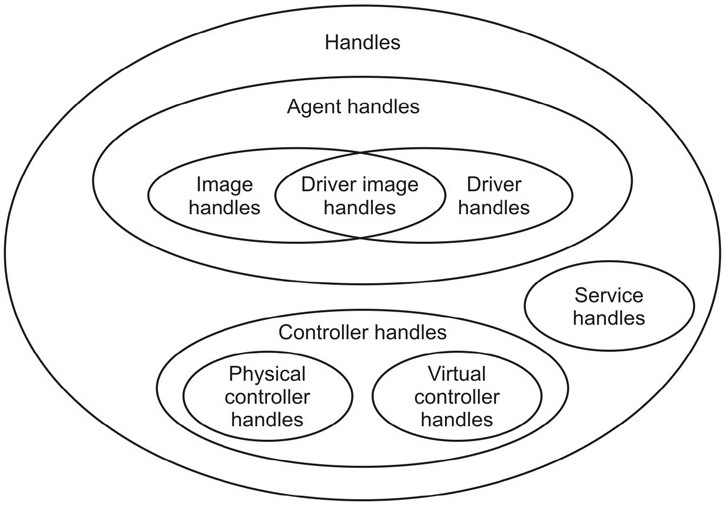
\includegraphics[width=0.7\textwidth]{uefi/handle_types}%
    \caption{Handle types (taken from \cite[Figure 3]{tianocore-edk2-driver-writer-s-guide})}%
    \label{fig:handle-types}%
\end{figure}

\cite{tianocore-edk2-driver-writer-s-guide} explains the categories of handles that are formed by the type of protocols that are grouped. \autoref{fig:handle-types} shows these categories.

\begin{description}
    \item[Image handles] are handles of \ac{UEFI} images loaded into memory, as they support the \hyperref[lst:loaded-image-protocol]{Loaded Image Protocol}, giving access to information about the image in memory. This includes the image's address, size, memory type, origin and optional load options.
    \item[Driver handles] are handles that group the \ac{UEFI} Driver Model related protocols (Driver Binding Protocol, the two Component Name Protocols and the two Driver Diagnostics Protocols)
    \item[Driver image handles] are \ac{UEFI} Driver Model related protocols installed onto images loaded in memory.
    \item[Agent handles] is a term used in the \ac{UEFI} Driver Model, they describe tracked consumers of other protocols.
    \item[Controller/Device handles] are interchangably used to refer to physical and virtual devices that offer \ac{I/O} abstraction protocols.
        Physical device handles support the Device Path Protocol for generic path/location information \cite[Section 10.2]{uefi-spec}.
    \item[Service handles] are used for generic hardware unrelated abstractions.
\end{description}

\TODO{\ac{I/O} abstractions}

\subsection{\acs{UEFI} Driver Model}

\cite[Section 2.5.2]{uefi-spec} describes the \acs{UEFI} Driver Model, it simplifies the design of device drivers by moving implementation of the device mangement and discovery into the firmware, leaving drivers with only the responsibility to offer interfaces for installation and removal.

We will focus on device drivers, these do not add any new device handles but instead offer protocol abstractions build upon already existing \ac{I/O} abstractions offered by bus drivers.
A driver following the \ac{UEFI} Driver Model is not allowed to interact with any hardware in its entry point and is instead required to install an instace of the Driver Binding Protocol on its own image handle.
The Loaded Image Protocol also offers a field where a driver can provide a function to unload itself.
It may also additionally install the confirguration or diagnostic related protocols.
Runtime drivers usually register a notification function that is triggered when an \ac{OS} loader calls \code{ExitBootServices}, this allows them to translate any allocated memory to their virtual addresses.

The firmware will try to connect device drivers to a controller by iterating over all instances of the Driver Binding Protocol in the handle database and calling the \code{Supported} function of the Driver Binding Protocol on a controller. The device driver then checks whether it supports the controller by for example looking for specific \ac{I/O} abstraction protocols, that it will want to laters use and further abstract.
If the driver supports the device the firmware will call the \code{Start} function of the Driver Binding Protocol to have the driver install its offered protocols on the controller handle.
This is done recursively as the newly installed device driver might now fullfill the requirements for another driver.
The firmware can also call the \code{Stop} of the Driver Binding Protocol function if it wants a driver to uninstall its protocol instance from a controller, an example for this would be another device driver wanting to exclusively manage a controller. This is done by tracking agents of protocols, in other words the drivers who consume a protocol.

\subsection{Systemtable}

The UEFI System Table is an important data structure, it provides access to system configuration information, generic boot and runtime services \cite[Section 3.3]{tianocore-edk2-driver-writer-s-guide}.
It also serves as the entrance in to the \ac{UEFI} environment, as a loaded images receives a only pointer to the system table as well as its image handle through its entry point. Although the Loaded Image Protocol provides and interface to hand optional load options to the image \cite{beyond-bios}.

\autoref{fig:uefi-system-table}


\TODO{during boot boot and runtime services are available}

\begin{figure}[htb]%
    \centering%
    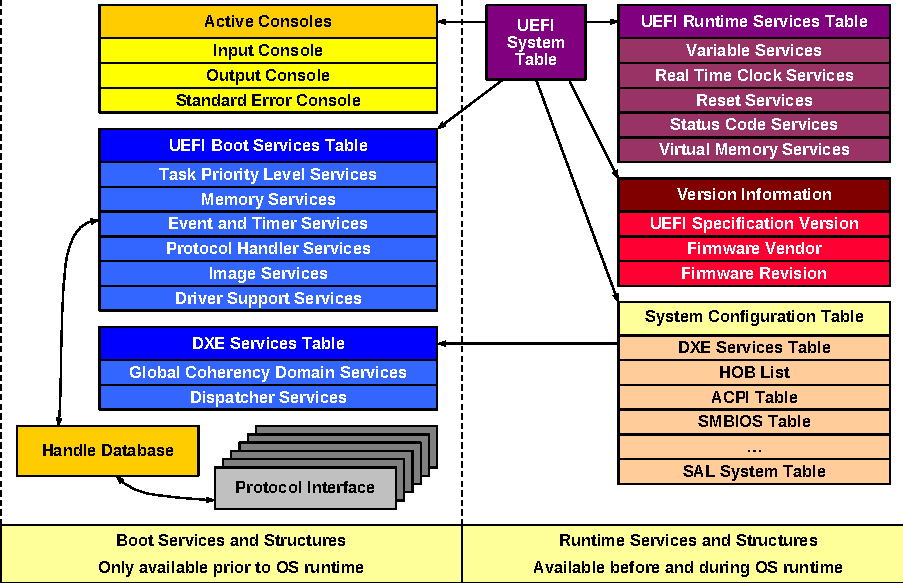
\includegraphics[width=0.8\textwidth]{uefi/uefi_system_table}%
    \caption{\ac{UEFI} System Table (taken from \cite[Vol 2, Figure 2-5]{pi-spec})}%
    \label{fig:uefi-system-table}%
\end{figure}


\subsubsection{Boot Services}

\ac{UEFI} applcations must use boot services functions to access devices and allocate memory. They are available until an \ac{OS} loader takes control over the system via a call to the boot service \code{ExitBootServices()}, from which on only runtime services are available. \cite[Section 7]{uefi-spec} splits the boot services into five categories:

\begin{description}
    \item [Event, Timer, and Task Priority Services] used to create, close, signal, wait for and check events. Setting timers and raising or restoring task priority levels.
    \item [Memory Allocation Services] to allocate and free pools or whole pages of memory, as well as retrieve the \ac{UEFI} managed memory map.
    \item [Protocol Handler Services] used to install, uninstall and retrieve protocol instance as well as abstractions related to the \ac{UEFI} Driver Model.
    \item [Image Services] to load, unload and start images. Images can also use these to transfer execution back to the firmware or with \code{ExitBootServices()} assume control over the system
    \item [Miscellaneous Services] offer basic memory manipulation, checksum calculation, watchdog timers and monotonic counters.
\end{description}

\subsubsection{Runtime Services}

\TODO{me}

\begin{description}
    \item [Variable Services] used to query, get and set \hyperref[sec:uefi-pi:uefi:variables]{variables}.
    \item [Time Services] used to get and set time as well as a system wakeup timer.
    \item [Virtual Memory Services] relate to enabling virtual memory and translating memory addresses.
    \item [Image Services] to load, unload and start images. Images can also use these to transfer execution back to the firmware or with \code{ExitBootServices()} assume control over the system
    \item [Miscellaneous Runtime Services] offer system reset, a monotonic counter and capsule services. Capsules allow the \ac{OS} to pass data to the firmware, this includes firmware managment related data.
\end{description}

\subsection{Variables}
\label{sec:uefi-pi:uefi:variables}

\ac{UEFI} variables are key/value pairs used to store arbitrary data passed between the \ac{UEFI} firmware and \ac{UEFI} applications.
The data type has to be known beforehand and as such is specified for variables defined in \ac{UEFI}.
The Storage implementation is not specified by \ac{UEFI}, but it must support non\-/volatility, to retain after reboots, or temper resistance if demanded.
Variables are defined by a vendor \ac{GUID}, a name and attributes.
Attributes include their scope (boot, runtime, non-volatile), whether writes require authentication or result in appending data instead of overwriting \cite[Section 8.2]{uefi-spec}.
Architecturally defined \ac{UEFI} variables are called Globally Defined Variables where the vendor \ac{GUID} has the value \code{EFI\_GLOBAL\_VARIABLE} \cite[Section 3.3]{uefi-spec}.

\subsection{Boot Manager}
\label{sec:uefi-pi:uefi:boot-manager}

The \ac{UEFI} boot manager is a firmware component executed after the platform is completely initialized, it decides which \ac{UEFI} drivers or applcations are loaded and when.
The boot behavior is configured through architecturally defined \ac{NVRAM} global variables\cite[Section 3.1]{uefi-spec}.
Each load option entry for a driver or application resides in a variable following the naming scheme of \code{Driver\#\#\#\#} or \code{Boot\#\#\#\#} respectively. Where \code{\#} stands for a hexadecimal digit forming a 4 digit number, requiring leading zeros.
If a firmware implementation allows for the creation of new load options they can then be added to the ordered lists \code{DriverOrder} and \code{BootOrder}, they reference load options and dictate the order in which they are processed.
Driver load options are processed before the boot load options, there also exists the \code{BootNext} variable to override the boot options once.
A general depiction of the \ac{UEFI} boot flow can be seen in \autoref{fig:uefi-boot-sequence}.
Implementations usually allow for an interactive menu, where users can modify the order or boot entries manually \cite[Section 3.1.1]{uefi-spec}.
Boot options are generally first attempted to be loaded through the \code{LoadImage} boot service.
If the device path of a boot option only points to a device instead to the file on a device, it attempts to load a default boot application with the \hyperref[lst:simple-file-system-protocol]{Simple File System Protocol}\cite[Section 3.1.2]{uefi-spec}, for x64 it uses the default path \code{\textbackslash EFI\textbackslash BOOT\textbackslash BOOTX64.EFI} \cite[Section 3.5]{uefi-spec}.

\begin{figure}[htb]%
    \centering%
    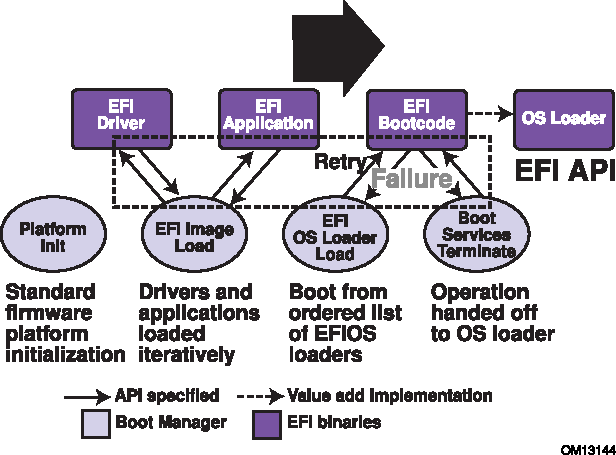
\includegraphics[width=0.8\textwidth]{uefi/uefi_boot_sequence}%
    \caption{Booting Sequence (taken from \cite[Figure 2-1]{uefi-spec})}%
    \label{fig:uefi-boot-sequence}%
\end{figure}

% !TeX root = ../../thesis.tex

\subsection{Secure Boot}

Secure Boot provides a secure hand-off from the firmware to 3rd party applications used for during the boot process, located on unsecure media \cite{tianocore-understanding-uefi-secure-boot-chain} \cite[Sections 32.2 and 32.5.1]{uefi-spec}.
It assumes the firmware to be a trusted entity and all 3rd party software to be untrusted, this includes images from hardware vendors in \ac{PCI} option \acp{ROM}, bootloader from \ac{OS} vendors and tools such as the \ac{UEFI} shell \cite{tianocore-understanding-uefi-secure-boot-chain}.
Digital signatures, embedded within the \ac{UEFI} images, can be used to authenticate origin and/or integrity \cite[Section 32.2]{uefi-spec}.
This is done through asymmetric signing, component provider must sign their executables with their private key and publish the public key.
The public keys are stored in a signature \ac{DB} and before execution the signed executable can be verified against the database.
Multiple signatures can be embedded within the same image \cite[Section 32.2.2]{uefi-spec}.
The signatures are created by first calculating a hash over select parts of the executable, leaving, for example, the signatures out of the hashed data and then signing it with a private key.
The output of this hashing is called a digest and the algorithm for obtaining the digest is defined in \cite{microsoft-pe-signature-format}.
Secure Boot also disallows legacy booting through the \ac{CSM}.

Secure Boot is managed through three components, a \ac{PK}, one or more \ac{KEK} and the signature \acp{DB}.

\begin{description}
    \item[\ac{PK}]
        The \ac{PK} establishes a trust relationship between platform owner and firmware, the public half is enrolled into the firmware.
        The private half represents platform ownership, as it can be used to change or delete the \ac{PK} as well as enroll or modify \acp{KEK}.
    \item[\ac{KEK}]
        The \ac{KEK} establishes a trust relationship between \ac{OS} and firmware, as its private half is used to modify the signature \acp{DB}.
    \item[Signature \acfp{DB}]
        Signature \acp{DB} contain image hashes and certificates, to either allow or deny execution of associated images.
\end{description}

Internally these are all implemented by authenticated variables, residing in tamper resistant non-volatile storage \cite[Section 32.3]{uefi-spec}.
The \ac{PK} is a simple variable where the \ac{KEK} and \ac{DB} are implemented through signature list data structures \cite[Section 32.4.1]{uefi-spec}, the variable services can be used to append entries or to read and write the list as a whole \cite[Sections 32.3.5 and 32.5.3]{uefi-spec}.
The variables are part of the \hyperref[sec:uefi-pi:uefi:variables]{Globally Defined Variables}, for each variavble also exist a variant reserved for default entries. These can be used by an \ac{OEM} to supply platform\-/defined values, used during Secure Boot initialization.
Their contents can be copied to their live versions, used during Secure Boot operation.
The current state of Secure Boot is also reflected within a secure variable \cite[Section 3.3]{uefi-spec}.

% https://papers.vx-underground.org/papers/Other/Advanced%20Malware/UEFI%20Secure%20Boot%20in%20Modern%20Computer%20Security%20Solutions.pdf
Users, who are physically present, may disable Secure Boot, enroll default or custom keys via an interactive menu. \TODO{find a good cite}

\TODO{maybe secure boot authorization process}

\subsection{Firmware Management}

\TODO{me}

% https://microsoft.github.io/mu/dyn/mu_tiano_plus/FmpDevicePkg/Docs/FmpDevicePkg_ReadMe/

provides
CapsuleUpdate()
QueryCapsuleCapabilities()
of the runtime services table
\clearpage
% !TeX root = ../../thesis.tex

\section{\acf{PI}}

\subsection{\acs{PI} Architecture Firmware Phases}

The \ac{PI} Architecture defines distinct phases.
focus will be on dxe and transient system load
\autoref{fig:pi-phases}



\begin{figure}[htb]%
    \centering%
    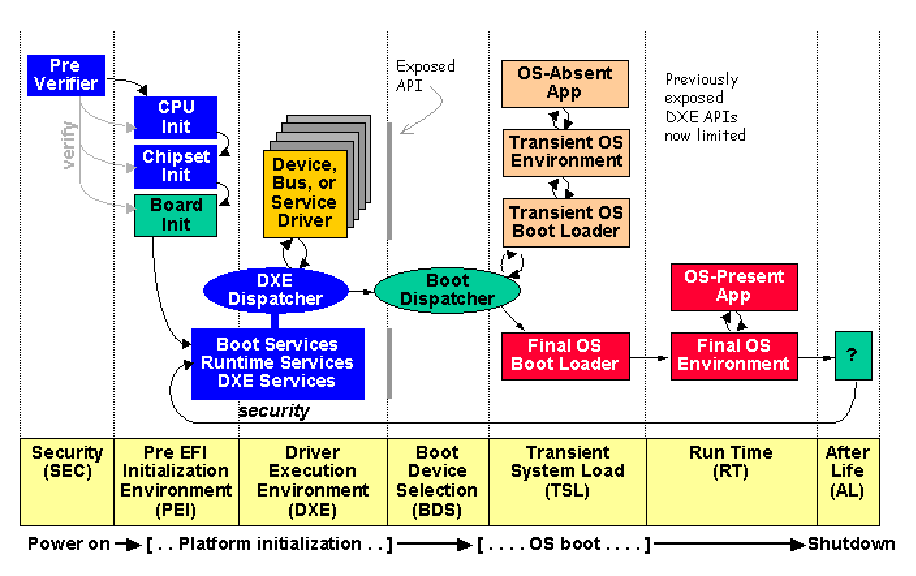
\includegraphics[width=\textwidth]{pi_boot_sequence}%
    \caption{\ac{PI} Architecture Firmware Phases \cite[Figure 2-1]{pi-spec}}%
    \label{fig:pi-phases}%
\end{figure}


\begin{enumerate}
    \item{\acf{SEC}}
    % % Since the CPU doesn't know about UEFI or BIOS the initial step is exactly the same, it starts in 16-bit real mode and fetches it's first instruction from `CS = 0xF000` and `IP = 0xFFF0` but instead of shifting `CS` left by four bits and adding `IP`, the `CS` base register is initialized to `0xFFFF'0000`. So the first instruction is fetched from the physical address `0xFFFF'FFF0` (`0xFFFF'0000 + 0xFFF0`). The CS base address remains at this initial value until the CS selector register is loaded by software (e.g. far jump or call instruction)

    % \begin{itemize}
    %     \item Populates Reset Vector Data structure
    %     \item Saves Built-in self-test (BIST) status
    %     \item Enables protected mode (16 bit -> 32 bit)
    %     \item Configures temporary RAM (not only limited in processor cache) by using MTRR to configure CAR.
    % \end{itemize}


    The \ac{SEC} phase is the first phase performed during platform initialization. Under its responsibilities fall handling all platform restart events, setting up temporary memory and establishing the system's root of trust. It serves as the foundation for all secure operations on which inductive security designs rely to build a chain of trust by having a module verify the integrity of its subsequent module. For this the \ac{SEC} phase may verify the integrity of the \ac{PEI} foundation before transfering execution to it. When it transfers execution, it also passes information about the current state of the system, including location and size of the temporary stack, \ac{RAM}, and \ac{BFV}. It can also optionally pass protocols for the \ac{PEI} phase to use.

    \item{\acf{PEI}}

    Configures a system meeting the minimum prerequisites for the Driver Execution (DXE) phase, which is generally a linear array of RAM large enough for successful execution.

    PEI provides a framework allowing vendors to supply initialization modules for each functionally distinct piece of system hardware which must be initialized before the DXE phase.

    PEI design goals of the PI architecture:
    \begin{itemize}
        \item Maintenance of the chain of trust, includes protection and authorization of PEI modules
        \item Provide a core PEI module
        \item Independent developement of intialization modules
    \end{itemize}
    The PEI phase consists of the PEI Foundation core and specialized plug-ins known as Pre-EFI Initialization Modules (PEIMs).

    Since the PEI phase is very early in the boot process it can't assume reasonable amounts of RAM so the features are limited:
    \begin{itemize}
        \item Locating, validating and dispatching PEIMs
        \item Communication between PEIMs
        \item Providing Hand-Off Data for DXE phase
        \item Initializing some permanent memory complement
        \item Describing the memory in Hand-Off Blocks (HOBs)
        \item Describing the firmware volume locations in HOBs
        \item Passing control into the Driver Execution Environment (DXE) phase
        \item Discover boot mode and possibly resume from sleep state
    \end{itemize}
    PEI Service Table visible to all PEIMs in the system, a pointer to this table is passed as an argument via the PEIM entry point, it is also part of each PEIM-to-PEIM Interface (PPI).


    % | Service                  | Description                                                                                                                                 |
    % | ------------------------ | ------------------------------------------------------------------------------------------------------------------------------------------- |
    % | PPI Services             | Manages PPIs to facilitate intermodule calls between PEIMs. Interfaces are installed and tracked on a database maintained in temporary RAM. |
    % | Boot Mode Services       | Manages the boot mode (S3, S5, normal boot, diagnostics, etc.) of the system                                                                |
    % | HOB Services             | Creates data structures called Hand-Off Blocks (HOBs) that are used to pass information to the next phase of the PI Architecture.           |
    % | Firmware Volume Services | Finds PEIMs and other firmware files in the firmware volumes                                                                                |
    % | PEI Memory Services      | Provides a collection of memory management services for use both before and after permanent memory has been discovered                      |
    % | Status Code Services     | Provides common progress and error code reporting services (for example, port 080h or a serial port for simple text output for debug).      |
    % | Reset Services           | Provides a common means by which to initiate a warm or cold restart of the system.                                                          |

    % #### PEI Foundation/Core

    PEI Foundation code is portable across all platforms of a given instruction-set. The set of exposed services is the same across different microarchitextures and allows PEIMs to be written in C.

    - Dispatches PEIMs
    - Maintains boot mode
    - Initializes permanent memory
    - Invokes DXE loader

    % #### PEI Dispatcher

    The PEI Dispatcher evaluates dependencies of PEIMs in the firmware volume, these dependencies are PPIs. The Dispatcher holds internal state machines to check dependencies of PEIMs, it starts executing PEIMs whose dependencies are statisfied to build up dependencies of other PEIMs, this is done until the dispatcher cannot invoke any more PEIMs. Then the DXE Initial Program Loader (IPL) PPI is invoked to pass control to the DXE phase.

    % #### Pre-EFI Initialization Modules (PEIMs)
    PEIMs are specialized drivers that personalize the PEI Foundation to the platform. They are analogus to DXE driver and generally correspond to the components being initialized. It is strongly recommended that PEIMS do only the minimum necessary work to initialize the system to a state that meets the prerequisites of the DXE phase. PEIMs reside in firmware volumes (FVs).

    % #### PEIM-to-PEIM Interfaces (PPIs)
    PEIMs communicate with each other using a structure called PPI. A PPI is a GUID pointer pair. The GUID is used to identifiy a certain service and the pointer provides access to data structures and services of the PPI.

    % There are two kinds of PPIs:
    % - Architectural PPIs
    % - Additional PPIs

    An architectural PPI is described in the PEI Core Interface Specification (CIS) and the GUID is known to the PEI Foundation. They typically provide a common interface to the PEI Foundation to a service with platform specific implementation.

    An additional PPI is important for interoperability but isn't required by the PEI Foundation, they can be classified as mandatory or optional.


    \begin{itemize}
        \item init permanent memory
        \item describe memory in \acp{HOB}
        \item describe \ac{FV} in \acp{HOB}
        \item pass control to \ac{DXE}
    \end{itemize}

    crisis recovery (what is this?)
    resuming from S3 sleep state
    linear array of RAM
    \ac{PEIM} provides a framework to allow vendors to supply separate initialization modules for
    each functionally distinct piece of system hardware that must be initialized prior to the DXE phase \cite{pi-spec}

    % design goals
    maintenance of chain of trust, protection against unauthorized updates to the PEI phase or modules
    authentication of the PEI Foundation and its modules
    provide core PEI module (PEI foundation) processor architecture independent, supports add-in moudles from vendors for processors, chipsets, RAM

    % what it does
    Locating, validating, and dispatching PEIMs
    Facilitating communication between PEIMs
    Providing handoff data to subsequent phases

    \item{\acf{DXE}}


    % - DXE Foundation/Core
    % - DXE Dispatcher
    % - DXE Drivers

    % #### DXE Foundation

    The DXE Foundation produces a set of Boot, Runtime and DXE Services and exposes them through handle databases in the EFI System Table. It is designed to be completely portable, independent of processor, chipset and platform. The only dependent of the Hand-Off Blocks from the PEI phase, after these are processed the all prior phases can be unloaded.

    % #### DXE Dispatcher

    The DXE Dispatcher discovers DXE drivers within the Firmware Volume (FV) and executes them in the correct order, respecting their dependencies towards each other. The Firmware Volume file format allows the DXE driver images to be packaged with expressions about their dependencies. Since the DXE Drivers are PE/COFF images the dispatcher comes with an apropriate loader to load and execute the image format.

    % #### DXE Drivers

    % - Drivers that execute very early in the DXE phase
    % - Drivers that comply with the UEFI Driver Model

    The DXE Drivers are responsible for initializing the processor, chipset,
    and platform components as well as providing software abstractions for console and
    boot devices in the form of services.

    dxe core/foundation
    platform independent
    is implementation of UEFI
    UEFI Boot Services
    UEFI Runtime Services
    DXE Services

    dxe dispatcher
    discover drivers stored in firmware volumes and execute in proper order
    apriori file optionally in FV or depex of driver
    after dispatching all drivers in the dispatch queue hands control over to BDS

    dxe drivers
    init processor, chipset and platform
    produce arichtectural protocols and \ac{I/O} abstractions for consoles and boot devices

    % responsibilities
    initializing the processor, chipset, and platform components
    providing software abstractions for system services, console devices, and boot devices.

    \item{\acf{BDS}}
    The DXE Foundation will hand control to the BDS Architectural Protocol after all of the DXE drivers whose dependencies have been satisfied have been loaded and executed by the DXE Dispatcher.

    % - Initializing console devices based on the ConIn, ConOut, and StdErr environment variables
    % - Loading device drivers listed in the DriverOrder environment variables
    % - Attempting to load and execute boot selections list from the BootOrder environment variables

    During the BDS phase new Firmware Volumes (FV) might be discovered and control is once again handed to the DXE Dispatcher to load drivers found on these additional volumes.


    DXE arichtectural protocol
    one function entry
    platform boot

    attempts to connect boot devices required to load the os
    discovers volumes containing new drivers
    calls DXE dispatcher
    doesnt return when successfully booting OS

    UEFI itself only specifies the NVRAM variables used in selecting boot options
    leaves the implementation of the menu system as value added implementation space \cite{uefi-spec}

    \cite{pi-spec}

    \begin{itemize}
        \item Initializing console devices
        \item Loading device drivers
        \item Attempting to load and execute boot selections
    \end{itemize}

    \item{\acf{TSL}}

    The Transient System Load (TSL) is primarily the OS vendor provided boot loader. Both the TSL and the Runtime Services (RT) phases may allow access to persistent content, via UEFI drivers and UEFI applications. Drivers in this category include PCI Option ROMs.

    This phase ends when an OS boot loader calls 'ExitBootServices()'.

    boot and runtime services/driver
    bootloader
    \cite[Section 13.3]{uefi-spec}
    \cite[Section 3.5.1.1]{uefi-spec}

    ExitBootServices()

    \item{\acf{RT}}
    Boot service drivers have been unloaded and only runtime services are accessible.


    runtime services/driver

    \item{\acf{AL}}
    The After Life (AL) phase consists of persistent UEFI drivers used for storing the state of the system during the OS orderly shutdown, sleep, hibernate or restart processes.

    hibernation
    sleep

\end{enumerate}

\subsection{\acs{UEFI}/\acs{PI} Firmware Images}

Firmware Images are stored in Flash Devices (FD), a Firmware Volume (FV) serves as file level interface. Usually multiple FVs are present in a single FD but a signle FV can also be distributed via multiple FDs.
A FV is formatted with a binary file system, typically with Firmware File System (FFS).

In a FFS modules are stored as files, they can be executed at the fixed address from Read Only Memory (ROM) or through relocation in loaded memory. Within a file are multiple sections which then contain the "leaf" images. These are for example PE32 images.

% https://edk2-docs.gitbook.io/edk-ii-build-specification/2_design_discussion/22_uefipi_firmware_images
\cite[Vol. 3, Section 2.1]{pi-spec}

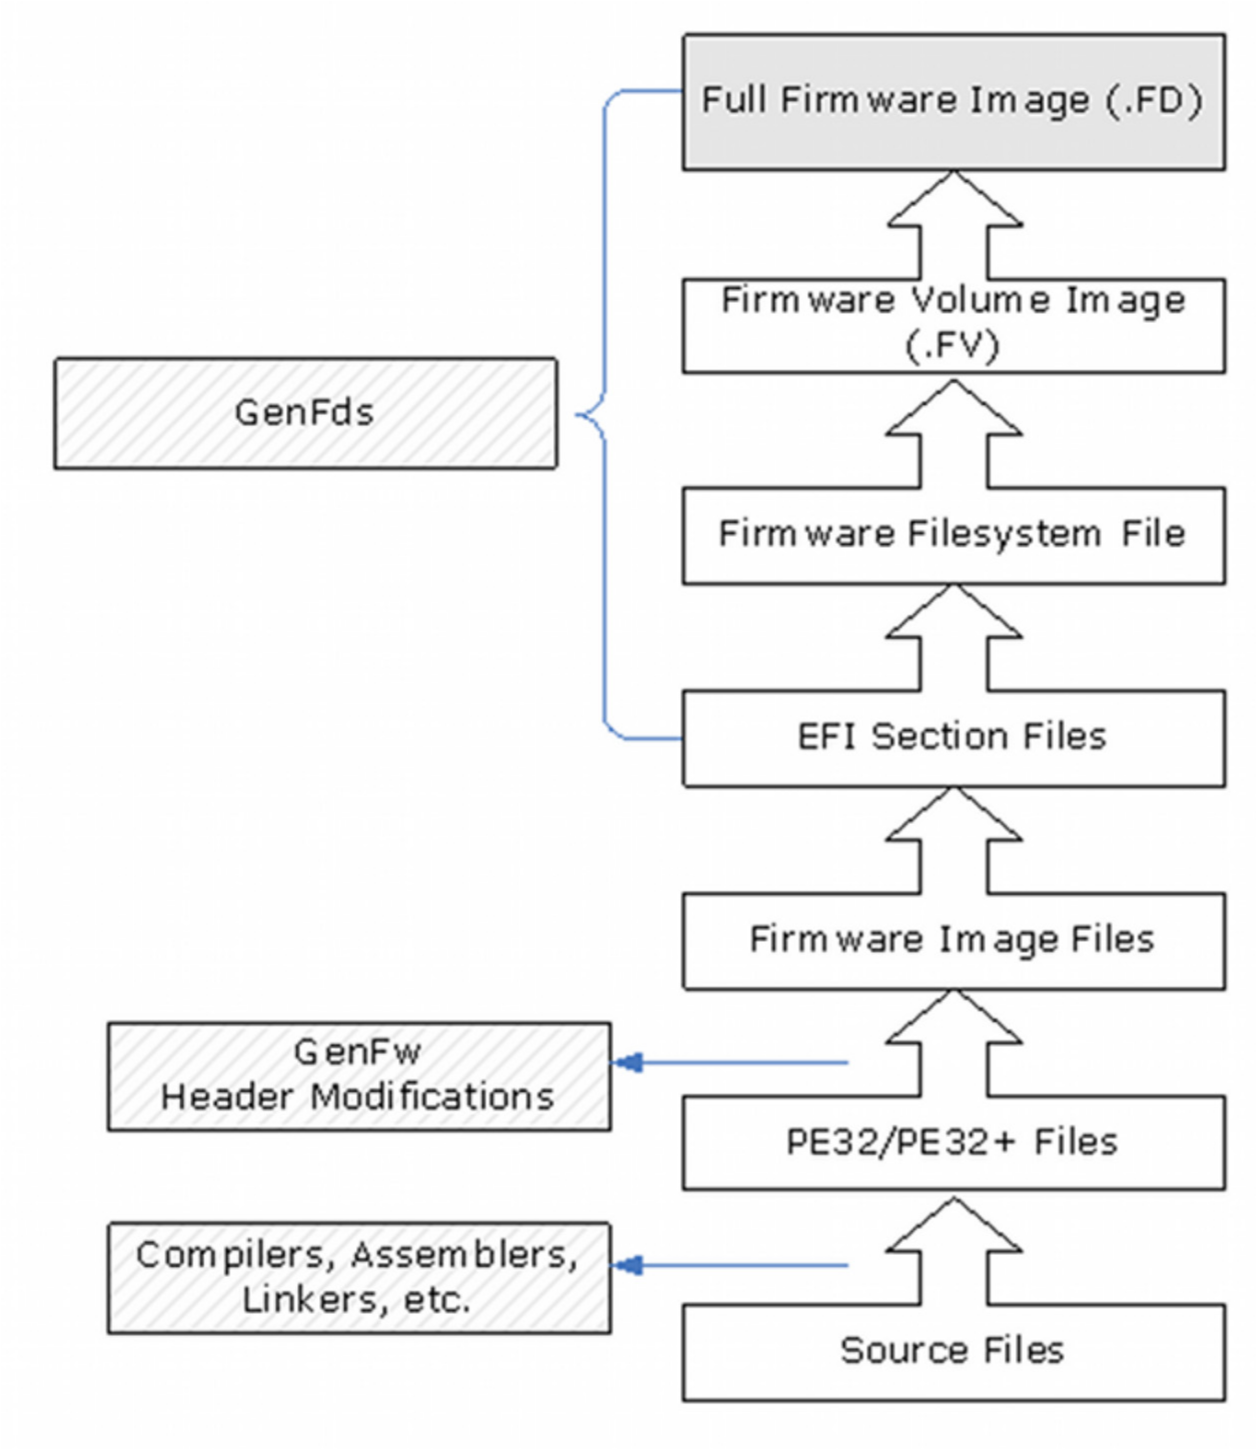
\includegraphics[width=\textwidth]{flash_device}
\ac{FD}
persistent
physical device
contains firmware code and/or data
typically flash
may be divided into smaller pieces to form multiple logical firmware devices
multiple physical firmware devices may be aggregated into one larger logical firmware device

\acf{FV}
logical device
organized into a file system
attributes such as
- size
- formatting
- read/write access

\acf{FFS}
organization of files and free space
no dierectory hierarchy
all files flat in root dir
parsing requires walking for beginning to end

firmware files
types
% PEI_CORE
% PEIM
% DXE_CORE
% DRIVER
% FIRMWARE_VOLUME_IMAGE
% FREEFORM

some file types are sub-divided in file sections

file sections can be either
encapsulation or leaf
leaf sections such as
PE32
% DXE_DEPEX
% PEI_DEPEX
RAW
VERSION
TE

dxe drivers files
contain one PE32 executable section
may contain version section
may contain dxe depex section

freeform files
can contain any combination of sections

PEI phase Service Table
FfsFindNextFile, FfsFindFileByName and FfsGetFileInfo

DXE phase
% EFI_FIRMWARE_VOLUME2_PROTOCOL

depex

\cite{tianocore-edk2-build-spec}

% !TeX root = ../../thesis.tex

\subsection{Security}
\label{sec:uefi-pi:pi:security}

The \ac{PI} specification defines \acp{PPI} and \ac{DXE} protocols which can be used to validate images when loading them.
During the \ac{PEI} phase, the \emph{\ac{PEI} Guided Section Extraction \ac{PPI}} can be used to authenticate file sections, while the \emph{Security \ac{PPI}} implements the policy response to the authentication result.
The \ac{DXE} phase has counter parts in the form of the \emph{Guided Section Extraction Protocol} and the \emph{Security Architectural Protocol}.
The policy response may be the locking of flash upon authentication failure or attestation logging \cite[Vol. 2, Section 12.9.1]{pi-spec}.
It also has the architectural protocol \emph{Security2 Architectural Protocol}, which implements Secure Boot validation, \ac{TCG} measured boot, and User Identity policy for image loading.
The implementation of the boot service \code{LoadImage()} has to use these protocols in accordance to the rules defined in \cite[Vol. 2, Section 12.9.2]{pi-spec}.
The Security2 protocol is invoked on every loaded image, with the Security protocol being invoked afterwards on images loaded through the Firmware Volume Protocol.
When the Security2 protocol is not installed it uses the Security protocol regardless of the image's origin.

\subsubsection{Hardware Validated Boot}

Secure Boot relies on the firmware as its root of trust.
Hardware validated boot is able to shift the root of trust out of the firmware image into a smaller part in the hardware, in hopes to reduce the size of the attack vector.
This part performs validation of the \ac{IBB} before handing over execution to the firmware image \cite{tianocore-understanding-uefi-secure-boot-chain}.

\subsubsection{Firmware Protection}

The \ac{PI} specification defines an \emph{End of \acs{DXE} Event}, which indicates the introduction of third party software execution to the platform.
Up until this point it is assumed that the entire system software is under the control of the platform manufacturer.
Drivers may react to this event by locking critical system resources, using the \ac{SMM} related services \cite[Vol. 2, 5.1.2.1]{pi-spec}.
The \ac{SMM} is a secure execution environment, achieved by isolation from the rest of the system, through the \ac{CPU} \cite[Vol. 4, Section 1.3]{pi-spec}.
The \ac{PI} reference implementation also makes use of this event to lock the device that stores the firmware image \cite{tianocore-edk2-fmpdxe}.


% !TeX root = ../../thesis.tex

\subsection{Security}
\label{sec:uefi-pi:pi:security}

The \ac{PI} specification defines \acp{PPI} and \ac{DXE} protocols which can be used to validate images when loading them.
During the \ac{PEI} phase, the \emph{\ac{PEI} Guided Section Extraction \ac{PPI}} can be used to authenticate file sections, while the \emph{Security \ac{PPI}} implements the policy response to the authentication result.
The \ac{DXE} phase has counter parts in the form of the \emph{Guided Section Extraction Protocol} and the \emph{Security Architectural Protocol}.
The policy response may be the locking of flash upon authentication failure or attestation logging \cite[Vol. 2, Section 12.9.1]{pi-spec}.
It also has the architectural protocol \emph{Security2 Architectural Protocol}, which implements Secure Boot validation, \ac{TCG} measured boot, and User Identity policy for image loading.
The implementation of the boot service \code{LoadImage()} has to use these protocols in accordance to the rules defined in \cite[Vol. 2, Section 12.9.2]{pi-spec}.
The Security2 protocol is invoked on every loaded image, with the Security protocol being invoked afterwards on images loaded through the Firmware Volume Protocol.
When the Security2 protocol is not installed it uses the Security protocol regardless of the image's origin.

\subsubsection{Hardware Validated Boot}

Secure Boot relies on the firmware as its root of trust.
Hardware validated boot is able to shift the root of trust out of the firmware image into a smaller part in the hardware, in hopes to reduce the size of the attack vector.
This part performs validation of the \ac{IBB} before handing over execution to the firmware image \cite{tianocore-understanding-uefi-secure-boot-chain}.

\subsubsection{Firmware Protection}

The \ac{PI} specification defines an \emph{End of \acs{DXE} Event}, which indicates the introduction of third party software execution to the platform.
Up until this point it is assumed that the entire system software is under the control of the platform manufacturer.
Drivers may react to this event by locking critical system resources, using the \ac{SMM} related services \cite[Vol. 2, 5.1.2.1]{pi-spec}.
The \ac{SMM} is a secure execution environment, achieved by isolation from the rest of the system, through the \ac{CPU} \cite[Vol. 4, Section 1.3]{pi-spec}.
The \ac{PI} reference implementation also makes use of this event to lock the device that stores the firmware image \cite{tianocore-edk2-fmpdxe}.

\clearpage
% !TeX root = ../../thesis.tex

\section{\acs{UEFI} Shell}

Part of the family of \ac{UEFI} specifications is a shell specification which defines a feature rich \ac{UEFI} shell application to interact with the \ac{UEFI} environment \cite[Section 1.1]{uefi-shell-spec}.
It offers commands relating to boot and general configuration, device and driver management, file system access, networking \cite[Section 5.1]{uefi-shell-spec} and scripting \cite[Section 4]{uefi-shell-spec}.
A shell application may already be part of the boot options but can always be supplied in the default boot path of removable media.

The \ac{UEFI} shell is a great tool to visualize the \ac{UEFI} environment.
With the \program{devtree} command, for example, we can see the tree of all handles complying to the \ac{UEFI} driver model.
This also serves a great reference of how device paths are formed.
\autoref{fig:devtree} shows the output of \program{devtree} cropped to show a \ac{GPT} formatted hard drive and its logical partitions.
When the firmware discovers a block device it is also required to search for a partition table and create a device handle for each partition.
Device drivers abstracting file systems can then be connected to a partition handle and check if it is formatted.
The first partition here, listed as \emph{FAT File System}, is the \ac{ESP} of this drive.

\begin{figure}[htb]
    \centering
    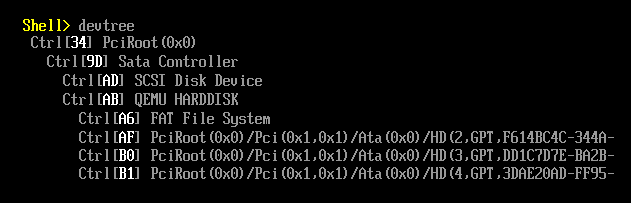
\includegraphics[width=1.0\textwidth]{uefi/devtree}
    \caption{Shortened \ac{UEFI} shell output of \program{devtree}}
    \label{fig:devtree}
\end{figure}

With \program{openinfo} we can see the group of protocols that a handle represents.
\autoref{fig:openinfo} shows the output when querying the handle of an \ac{ESP}.
Since this \ac{ESP} is installed in a logical partition an instance of the Partition Information Protocol is present.
The command also lists the agent handles of each protocol and how the protocol was accessed.
\code{TestProt} is often used in the \code{Supported} function of a driver, while \code{GetProt} is then used to open the protocol for consumption within the \code{Start} function.

\begin{figure}[htb]
    \centering
    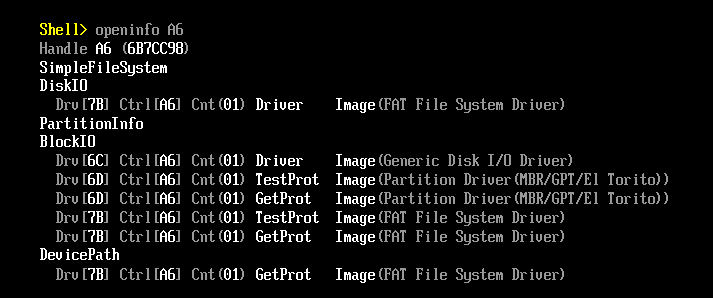
\includegraphics[width=1.0\textwidth]{uefi/openinfo}
    \caption{Shortened \ac{UEFI} shell output of \program{openinfo}}
    \label{fig:openinfo}
\end{figure}



% During initialization the shell produces default mappings for file systems and block devices, this defines names that can be used interchangably with their device paths when issuing shell commands \cite[Section 3.7.2]{uefi-shell-spec}.
% These mappings are designed to be consistent across reboots as long as the hardware configuration stays the same, they are comparable to Windows partition letters \cite[Appendix A]{uefi-shell-spec}.
% It also produces the initial output of what is equivalent to the invocation of the commands \program{ver} and \program{map} \cite[Section 3.3]{uefi-shell-spec}.
% \program{ver} displays the version of the \ac{UEFI} specification the firmware conforms to, while map shows the current device mapping \cite[Section 5.3]{uefi-shell-spec}.
% \autoref{fig:uefi-shell} depicts an exemplary output of the \ac{EDK} II \ac{UEFI} shell.

% When we inspect the mapping table we can see \lstinline{FSx:} and \lstinline{BLKx:} aliases, \lstinline{FSx:} maps to file systems and \lstinline{BLKx:} to block devices.
% This identification is performed via instances of the \hyperref[lst:simple-file-system-protocol]{Simple File System Protocol} and \TODO{double check} Block \ac{I/O} Protocol.
% % explain Simple File System Protocol
% The \hyperref[lst:simple-file-system-protocol]{Simple File System Protocol} \cite[Section 13.4]{uefi-spec} provides, together with the \hyperref[lst:simple-file-system-protocol]{File Protocol}, file-type access to the device it is installed on \cite[Section 13.5]{uefi-spec}.
% The two protocols are independent of the underlying file system the media is formatted with.


\section{\acs{EDK} II}

\ac{EDK} II, maintained by \emph{TianoCore}, is an open source implementation of \ac{UEFI}, offering a modern, feature-rich, cross-platform firmware development environment for the \ac{UEFI} and \ac{PI} specifications \cite{tianocore}.
It can be used to build modules of all types defined in the \ac{PI} and \ac{UEFI} specification and supports the generation of \ac{PF} images, option\-/\acp{ROM} and bootable media.
On top of implementing the \ac{PI} and \ac{UEFI} specifications, it defines a lot of helpful libraries and protocols that can be used to simplify the development process.
With events that require policiy defined reactions, it often already offers well\-/defined interfaces for a platform designer to pick up on.
The build process is flexible, as it can use different compilers such as \program{GCC} and \program{MSVC}.

\emph{TianoCore} also offers a lot of material to learn about developing applications, drivers, firmware, and a general understanding about the \ac{UEFI} ecosystem.
% !TeX root = ../thesis.tex

\chapter{Windows 11}

\TODO{what is 11 compared to 10}

\section{Installation}

For us to understand how UEFI threats act towards Windows we need to understand how the layout of the Windows installation integrates into the UEFI environment.
% uefi begins with windows installation
This begins with the installation process and the partitioning of the hard drive Windows is installed onto.
% creates at least four partitions
When the Windows Installer is launched, it creates at least four partitions on the target hard drive.
The \acf{ESP}, a recovery partition, a partition reserved for temporary storage and the boot partition containing the system files.
Two copies of the Windows Boot Manager \lstinline{bootmgfw.efi} are placed on the \ac{ESP}, one under \lstinline{EFI\\Boot\\bootx64.efi} for the default boot behavior the installed hard drive and one under \lstinline{EFI\\Microsoft\\Boot\\bootmgfw.efi} alongside boot resources such as the \ac{BCD}.
The path of the latter boot manager is saved in a boot load option variable entry \lstinline{Boot####}, which is then added to the \lstinline{BootOrder} list variable.
The boot load option contains optional data consiting of a GUID identifying the Windows Boot Manager entry in the \ac{BCD}.
The \ac{BCD}, as its name suggests, contains arguments used to configure various steps of the boot process \cite[12. The Windows Boot Manager]{windows-internals-7-part2}.
The boot partition is the primary Windows partition and is formatted with the \ac{NTFS} file system containing the Windows installation.
This is also the location of the final step of the Windows UEFI boot process, \lstinline{Windload.efi}, the application repsonsible for loading the kernel into memory \cite[12. The Windows OS Loader]{windows-internals-7-part2}.

\section{Boot Process}

Now that we established the basic structure of the Windows UEFI boot environment, we can discuss the boot process.
The Windows boot process begins after the UEFI Boot Manager launches the Windows Boot Manager, which starts by retrieving its own executable path and the \ac{BCD} entry GUID from the boot load options.
Then it loads the \ac{BCD} and access its entry.
If not disabled in the \ac{BCD} it loads its own executable into memory for integrity verification \cite[12. The Windows Boot Manager]{windows-internals-7-part2}.
Depending on what hibernation status is set within the \ac{BCD} it may launch the \lstinline{Winresume.efi} application, which reads the hibernation file and resumes kernel execution \cite[12. Launching a boot application]{windows-internals-7-part2}.
On a full boot it checks the \ac{BCD} for boot entries, if the entry points to a BitLocker encrypted drive, it attempts decryption.
If this faile it will show a reocvery prompt, otherwise it proceeds to load the \lstinline{Windload.efi} \ac{OS} loader \cite[12. Launching a boot application]{windows-internals-7-part2}.

% tries to TPM unseal
% url and message are read from BCD
% if succeeds make sure TPM cant be used to unseal further things
% StartImage os loader, only returns in error case
% if so start Windows Recovery Sequence
\TODO{TPM interaction}
\cite[12. Launching a boot application]{windows-internals-7-part2}


\section{Registry}

A crucial part to the whole Windows ecosystem is the Registry, it is a system database containing information required to boot, such as what drivers to load, general system wide configuration as well as application configuration.
\cite[1. Registry]{windows-internals-7-part1}
The Registry is a hierachical database containing keys and values, keys can contain other keys or values, forming a tree structure.
Values store data through various data types.
It is comparable to a file system structure with keys behaving like directories and values like files \cite[10. The registry - Registry data types]{windows-internals-7-part2}.
At the top level it has 9 different keys \cite[10. The registry - Registry logical structure]{windows-internals-7-part2}.
Normally Windows users are not required to change Registry values directly and instead interact with it through applications providing setting abstractions.
Though some more advanced options may not be exposed and can be accessed through the \lstinline{regedit.exe} application which provides a graphical user interface to travere and modify the Registry \cite[10. The registry - Viewing and changing the registry]{windows-internals-7-part2}.
It also supports ex- and importing registry keys along their subkeys and contained values.
Internally the registry is not a single large file but instead a set of file called hives, each hive contains one tree, that is mapped into the Registry as a whole.
There is no one to one mapping of registry root key to hive file, the \ac{BCD} file for example is also a hive file and is mapped into the Registry under \lstinline{HKEY_LOCAL_MACHINE\BCD00000000} \cite[10. The registry - Registry logical structure]{windows-internals-7-part2}.
Some hives even reside entirely in memory as a means of offering hardware configuration through the Registry \ac{API}.

\TODO{maybe fun fact that EFS cant encrypt hives}
windows also has a feature called Encrypting File System (EFS) with file system level encryption but it cant be used for registry hives
\cite[9. BitLocker Drive encryption]{windows-internals-6-part2}


% https://learn.microsoft.com/en-us/windows/whats-new/windows-11-overview#security-and-scanning
% \subsection{User Access Control (UAC)}
% https://learn.microsoft.com/en-us/windows/security/identity-protection/user-account-control/how-user-account-control-works

\section{Trusted Boot}
% https://learn.microsoft.com/en-us/windows/security/information-protection/secure-the-windows-10-boot-process
% https://learn.microsoft.com/en-us/windows/security/trusted-boot
% https://www.anoopcnair.com/understanding-windows-trusted-boot/
\subsection{KMCI}
\subsection{HVCI}
% https://learn.microsoft.com/en-us/windows-hardware/design/device-experiences/oem-hvci-enablement

\section{\acf{BDE}}
\label{sec:bde}
Windows is only able to enforce security policies when it is active, leaving the system vulnerable when accessed from outside of the \ac{OS} \cite[9. BitLocker Drive encryption]{windows-internals-6-part2}.
Windows uses BitLocker, integrated \ac{FVE}, aimed to protect system files and data from unauthorized accecss while at rest \cite{microsoft-bitlocker-overview}, while also verifying boot integrity when used with a \ac{TPM} \cite[9. BitLocker Drive encryption]{windows-internals-6-part2}.
The en- and decryption of the volume is done by a filter driver beneath the \ac{NTFS} driver as shown in \autoref{fig:bitlocker-volume-access-driver-stack}.
The \ac{NTFS} driver translates file and directory access into block-wise operations on the volume \TODO{CITE}, the filter driver receives these block operations, encrypting blocks on write and decrypting blocks on read, while they pass through.
This leaves the en- and decryption entirely transparent, making the underlying volume appear decrypted to the \ac{NTFS} driver \cite[9. Full-Volume Encryption Driver]{windows-internals-6-part2}.
The encryption of each block is done using a modified version of the \ac{AES}128 and \ac{AES}256 cypher \cite[9. Encryption Keys]{windows-internals-6-part2}.
A \ac{FVEK} is used in combination with the block index as input for the algorithm, resulting in an entirely different output for two blocks with identical data \cite[9. Full-Volume Encryption Driver]{windows-internals-6-part2}.
The \ac{FVEK} is encrypted with a \ac{VMK} which is in turn encrypted with multiple protectors, these encrypted versions of the \ac{VMK} are stored together with the encrypted \ac{FVEK} in an unencrypted meta data portion at the beginning of the volume \cite[9. Encryption Keys]{windows-internals-6-part2}.
The \ac{VMK} is encrypted by the following protectors:

\begin{itemize}
    \item[Startup key] stored in a \lstinline{.bek} file with a \ac{GUID} name equaling key identifier in bitlocker meta data
        \cite[2.6. Startup key]{bde-format-spec}
    \item[TPM]
        - tpm only
        no additional user interaction
        - tpm with startup key
        additional usb
        - tpm with PIN
        - tpm with startup key and PIN
        \cite{microsoft-bitlocker-countermeasures}
        with tpm ensures integrity of early boot components and boot configuration
        tpm usage requires \ac{TCG}2 compliant \ac{UEFI} firmware \cite[9. TPM]{windows-internals-6-part2}

        tpm is used to \emph{seal} and \emph{unseal} \ac{VMK}
        \TODO{PCR table either here or at TPM section}
        platform validation profile
        default \acp{PCR} are 0, 2, 4, 5, 8, 9, 10 and 11
        11 is required
    \item[Recovery key] recovery key 48 digits of 8 blocks
        block is converted to a 16-bit value making up a 128-bit key
        \cite[2.4. Recovery key]{bde-format-spec}
        % how to obtain
        when enabling manually, save on non encrypted medium
        \cite{microsoft-bitlocker-basic-deployment}

        bitlocker device encryption if supported automatically enabled
        after clean install encrypted with clear key (bitlocker suspended state)
        non domain account -> recovery key uploaded to microsoft account
        domain account -> recovery key backed up to active directory domain services (AD DS)
        clear key removed
        \cite{microsoft-bitlocker-device-encryption}

    \item[User key] password with max 49 characters
        \cite[2.7. User key]{bde-format-spec}
    \item[Clear key] unprotected 256-bit key stored on the volume to decrypt vmk
        \cite[2.5. Clear key]{bde-format-spec}
        used for suspension


        \TODO{decide if we add this} With Windows 11 and Windows 10, administrators can turn on BitLocker and the TPM from within the Windows Pre-installation Environment \cite{microsoft-bitlocker-device-encryption}

        \begin{figure}[htb]%
            \centering
            \includesvg{bitlocker_volume_access_driver_stack.drawio.svg}
            \caption{BitLocker Volume Access Driver Stack, inspired by \cite[Figure 9-24]{windows-internals-6-part2}}%
            \label{fig:bitlocker-volume-access-driver-stack}%
        \end{figure}

\end{itemize}
% !TEX root = ../thesis.tex

\chapter{Past Threats}
\label{sec:past-threats}

% https://www.blackhat.com/docs/asia-17/materials/asia-17-Matrosov-The-UEFI-Firmware-Rootkits-Myths-And-Reality.pdf
% https://www.researchgate.net/profile/Anton-Sergeev-2/publication/269310822_Too_young_to_be_secure_Analysis_of_UEFI_threats_and_vulnerabilities/links/551306b50cf23203199aa237/Too-young-to-be-secure-Analysis-of-UEFI-threats-and-vulnerabilities.pdf

Before we implement our \ac{UEFI} attacks, we first take a look at how past \ac{UEFI} threats are structured.
The threats discussed range from actual attacks found in the wild and analyzed by security researchers, over attacks that have been implemented for similar research purposes, to tools that enable system owners a more advanced control over their systems.


\begin{center}
    \begin{tabular}{lll}
        \toprule
        \textbf{Approach}                  & \textbf{Bootkit} & \textbf{Rootkit} \\
        \arrayrulecolor{gray}
        \cmidrule[0.4pt](r){1-1}
        \cmidrule[0.4pt](lr){2-2}
        \cmidrule[0.4pt](l){3-3}
        \multirow{4}{4em}{Storage\-/based} & \textbf{ours}    & VectorEDK        \\
                                           &                  & Mosaicregressor  \\
                                           &                  & LoJax            \\
                                           &                  & \textbf{ours}    \\
        \cmidrule[0.4pt](r){1-1}
        \cmidrule[0.4pt](lr){2-2}
        \cmidrule[0.4pt](l){3-3}
        \multirow{3}{4em}{Memory\-/based}  & Efiguard         & MoonBounce       \\
                                           & ESPecter         & CosmicStrand     \\
                                           & Dreamboot        &                  \\
                                           & FinSpy           &                  \\
        \arrayrulecolor{black}
        \bottomrule
    \end{tabular}
\end{center}

\section{Infection}
\vspace{-0.5em}

The infection is the most important part of an attack, as it dictates when, in what environment, and with what privileges the \ac{UEFI} payload is executed.

\vspace{-0.5em}
\subsection{Bootkit}
\vspace{-0.5em}

Bootkits use the \ac{UEFI} Boot manager to gain execution on a system.
There are a variety of methods using different mechanisms of the boot process.
FinSpy backs up and replaces the Windows Boot Manager \program{bootmgfw.efi} on the \ac{ESP} \cite{finspy}.
ESPecter patches the entry point of the Windows Boot Manager \program{bootmgfw.efi} and its copy \program{bootx64.efi} located in the default boot path, so it executes malicious code upon launch \cite{especter}.
Dreamboot and EFIGuard are more proof-of-concept than real attacks and suggest being booted into using removable media, but they are also able to be added to the default boot path on an \ac{ESP}, or generally added as their own new boot entry \cite{efiguard}.
They are both applications, which launch the Windows Boot Manager through its boot entry upon execution \cite{dreamboot, efiguard}.

\subsection{Rootkit}

Firmware rootkits have been rarer and how exactly the firmware images were infected is not often known.
VectorEDK uses \ac{OEM}'s software tooling to generate a firmware update utility on a bootable \ac{USB} stick that can then be inserted with physical access to the system \cite{mosaicregressor}.

LoJax's infection method comes with a signed kernel driver from the program \program{RWEverything}.
\program{RWEverything} is a legitimate tool that can be used to query hardware\-/related information on a system.
LoJax uses the driver to read and write to memory mapped \ac{I/O}, as well as \ac{PCI} configuration registers.
It leverages this to find the \ac{SPI} flash mapping and dump the firmware image.
It then removes previously packaged \ac{NTFS} drivers and adds its payload.
Reflashing the modified image relies on the platform to be either misconfigured or of an older kind that has a race condition exploit.
The \ac{SPI} flash is secured by a \ac{BIOS} control register, which has a \ac{BIOS} Write Enable bit and \ac{BIOS} Lock Enable bit.
The locking mechanism has to be correctly implemented by firmware designers through \ac{SMM} interrupts.
When writing to the \ac{BIOS} Write Enable bit, while the \ac{BIOS} is enabled, the operation initially succeeds but is then reverted by a \ac{SMM} interrupt routine.
This could either be incorrectly implemented or exploited on older hardware through a race condition using multi\-/processing or multi\-/threading.
When one thread constantly sets the Write Enable bit to 1 and the other tries to perform write operations on the \ac{SPI} flash, the firmware image will eventually be overwritten \cite{lojax}.

MosaicRegressor and LoJax add their payload in the form of \ac{DXE} drivers to a firmware volume \cite{mosaicregressor-technical-details,lojax}, as these are automatically executed by the \ac{DXE} dispatcher.
MoonBounce and CosmicStrand instead patch existing files in the firmware image.
MoonBounce patches the \ac{DXE} Core \cite{moonbounce}, while CosmicStrand patches a \ac{DXE} driver \cite{cosmicstrand}.
While both approaches could fundamentally be done in the form of an added \ac{DXE} driver, it does make the detection harder.

\section{Approach}

We can categorize the threats by their attack vector.
Rootkits and bootkits do not seem to have distinct approaches, as they both start their execution in the \ac{UEFI} environment before the Windows boot process.
We found that their approach can mainly be divided into storage\-/based and memory\-/based attacks.
Storage\-/based attacks mostly gain execution in the operating system environment by writing their payload into the Windows installation and modifying configuration data on the disk.
These attacks are often performed offline before any parts of the operating system are executed.
Memory\-/based attacks instead hook into the operating system's boot process to execute malicious code alongside the operating system in memory.
For storage\-/based attacks, we were only able to find examples of rootkits \cite{vector-edk,mosaicregressor-technical-details,lojax}, whereas memory\-/based attacks were performed by both root- and bootkits \cite{dreamboot,efiguard,especter,finspy,moonbounce,cosmicstrand}.
There is no technical limitation as we show in \autoref{sec:attacks:neither:bootkit} when we implement our own storage\-/based bootkit, but more likely a general preference for memory\-/based attacks, as they are more sophisticated.
Storage\-/based attacks face more restrictions such as BitLocker and code integrity checks.

\subsection{Storage-based}

Storage\-/based attacks need file\-/based access to the Windows installation to modify its content.
The primary partition is \ac{NTFS} formatted and, due to the \ac{UEFI} specification only mandating compliant firmware to support \ac{FAT}12, \ac{FAT}16 and \ac{FAT}32 \cite[Section 13.3.1.1]{uefi-spec}, \ac{NTFS} drivers are delivered as part of the attack.
MosaicRegressor and Lojax seem to use VectorEDK's leaked \ac{NTFS} driver \cite{mosaicregressor-technical-details, lojax}.
LoJax deploys its payload under the file path \program{C:\brackslash Windows\brackslash SysWOW64\brackslash autoche.exe} and then modifies the registry entry \program{HKEY\underbreak LOCAL\underbreak MACHINE\brackslash SYSTEM\brackslash CurrentControlSet\brackslash Control\brackslash Session Manager\brackslash BootExecute}, so that its payload is executed instead of the original executable \cite{lojax}.
MosaicRegressor simply deploys its payload in the Windows startup folder \cite{mosaicregressor-technical-details}, whose contents, as its name suggests, are executed upon Windows startup.

\subsection{Memory-based}

It seems to be unique to ESPecter to patch out the integrity self-check of the Windows Boot Manager, as it is the only bootkit to change the bootloader on disk instead of in\-/memory \cite{especter}.
FinSpy and Dreamboot when executed, load \program{bootmgfw.efi} into memory and apply patches before transferring execution \cite{finspy, dreamboot}.
EFIGuard loads an additional \ac{UEFI} driver which hooks the boot service \code{LoadImage()}.
When the function is called to load \program{bootmgfw.efi}, it patches the bootloader in memory \cite{efiguard}.
MoonBounce applies its patches from within an \code{ExitBootServices()} hook \cite{moonbounce}.

The general approach is the same for all memory\-/based attacks.
They propagate malicious code execution further up in the boot chain by hooking each image of the boot process as it is loaded into memory, i.e., from \program{bootmgfw.efi} to \program{Winload.efi} to \program{ntoskernel.exe}, the kernel image.

EFIGuard and ESPecter patch the kernel to disable Windows Driver signing, allowing them to install further kernel drivers \cite{efiguard,especter}.
While FinSpy and Dreamboot deploy payloads executed with elevated privileges \cite{finspy,dreamboot}.
MoonBounce and CosmicStrand map code directly into the kernel space \cite{moonbounce,cosmicstrand}.
% !TeX root = ../thesis.tex

\chapter{Test Setup}
\label{sec:test-setup}

We perform our attacks against Windows 11 on three different setups.
Even though all three \ac{UEFI} firmwares are \ac{PI} specification compliant, there is still a lot of freedom for \acp{OEM}, when implementing the \ac{PF}.

\section{\acs{QEMU}}
\label{sec:test-setup:qemu}

Our main development setup is an emulated environment using the emulator \program{\ac{QEMU}} \cite{qemu} together with the \ac{OVMF} image, from \ac{EDK} II using version \code{edk2-stable202208}.
For Secure Boot we generate our own \ac{PK} and use the \emph{Microsoft Corporation \acs{KEK} \acsu{CA} 2011} and the two signature \acp{DB} \emph{Microsoft Windows Production PCA 2011} and \emph{Microsoft Corporation UEFI CA 2011} provided by Microsoft.
For BitLocker and to fullfill Windows 11's general requirement that a \ac{TPM} 2.0 is present, we use \program{swtpm}.
A \ac{TPM} emulated in software \cite{swtpm}.
Accessing the firmware image with this setup is done through simple file access.

\section{Lenovo Ideapad 5 Pro-16ACH6}
\label{sec:test-setup:lenovo}

Our first hardware setup is a Lenovo Ideapad 5 Pro-16ACH6, an \ac{AMD} based laptop with a \ac{AMD} Ryzen 9 5900H \cite{lenovo-ideapad}.
It supports Microsoft Device Guard and \ac{PCR}7 binding when Secure Boot is enabled.
We can read and write the firmware image with physical hardware access by using an \ac{SPI} flash programmer in combination with the Linux utility \program{flashrom}.

\section{ASRock A520M-HVS}
\label{sec:test-setup:asrock}

Our second hardware setup is a desktop \ac{PC} with an \ac{AMD} based ASRock A520M-HVS motherboard.
We use the lastest firmware image as of writing which is of version 2.30.
This setup also supports \ac{PCR}7 binding when Secure Boot is enabled.
The \ac{SPI} flash chip on the main board is disabled and instead an \program{EM100} \ac{SPI} flash emulator is attached.
When the system thinks it is accessing the \ac{SPI} flash chip, it is instead communicating with the emulator.
Additionally by dualbooting into Linux we can use \program{flashrom} to communicate with the \ac{SPI} chip for read and write access.
The Linux distribution of our choice, Ubuntu uses a so called Lockdown Mode when Secure Boot is enabled.
This blocks direct access to the \ac{SPI} chip \cite{man-kernel-lockdown}, but can be disabled while Secure Boot remains enabled \cite{disable-kernel-lockdown}.

% !TEX root = ../thesis.tex

\chapter{Attacks}
% chapter summary, briefly introduce the three attacks
Our different attacks face three escalating levels of security mechanisms. The first is with Secure Boot and Bitlocker disabled, the second is just Secure Boot enabled and the third is both Secure Boot and Bitlocker enabled with the focus of the study on Bitlocker.
% common assumption/requirement across the attacks
All attacks share the requirement of being able to add DXE Drivers to the DXE Volume.
% how to achieve assumption/requirement
This can be achieved by having read/write access to the SPI flash or using the Signed Capsule Update. Gaining read/write access to the SPI Flash is possible either through physical access to the device by using an SPI clamp on the chip itself or through exploits like for example the
% see SMM multi threaded exploit
. Signed Capsule Updates can be leveraged with access to private vendor information by signing the payload to make it appear legitimate or by intercepting the distribution process and employing infected firmware.
% ref lenovo vantage for distributed example
% network boot maybe

\section{Test Setup}
\TODO{describe test setup}


% !TeX root = ../../thesis.tex

\section{Neither Secure Boot nor Bitlocker}
use read access to dump image
% ref to background UEFI/PI IMAGE
since it an FV with FFS we can open with UEFITool
remove previous NTFS driver if present, for full control, might be read only etc
in UEFITool search and remove
add in NTFS driver
use write access

try in EFI shell
navigate to Windows folder
create folder

how does one compile uefi application with edk2
it's open source so we can look up examples for most stuff

try in code
compile dxe driver within ovmf to receive .ffs file with version depex user interface section
SimpleFileSystem Protocol iteration
write failed on hibernated file
patch to allow write on hibernated drives

pack executable binary as uefi module
edk2 produces freeform image with one raw section
iterate over firmware volume protocols
search for payload guid
check size match
override notepad works

% ref to background UAC signed
but no automatic execution nor elevated privileges
dll proxying
dll hijacking
registry editing

Task Scheduler
defined in xml
cached in registry
edit with start cmd.exe and trigger manually
whoami

chntpw and reged
port to uefi
edit Task in machine under Control
maybe look if just adding a key would have also worked
export target registry key
modify so that registry key can differ and found via matching values
import and override registry key on target machine
payload whoami
localsystem


% !TeX root = ../../thesis.tex

\section{Secure Boot Enabled}
\label{sec:attacks:secure-boot}

Our second attack is performed with Secure Boot enabled.
We assume that the signature \acp{DB} of allowed images does not contain our image's hashes and that the interactive \ac{UEFI} setup menu is password protected.
Otherwise, we could simply turn off Secure Boot.

\subsection{Bootkit}

The interactive menu being password\-/protected makes the likelihood of infection via booting into our installer smaller.
We now solely rely on the boot order/firmware policy to prefer removable media.
Even if this was to be the case, we promptly see that Secure Boot already denies the execution of the installer when trying to boot it.
When using our Windows installer we observe the same denial for the bootkit itself.
The Windows Boot Manager boot option pointing to our bootkit is now denied execution.
If we were to have overwritten the standard boot entry of the hard drive \program{EFI\brackslash Boot\brackslash bootx64.efi}, a copy of the Windows Boot Manager, Windows would now be rendered unbootable.

\subsection{Rootkit}

In \autoref{sec:uefi-pi:pi:security} we discussed how the \ac{PI} specification defines the usage of its two security architectural protocols, with them being required to be invoked on every call to \code{LoadImage()}, and that the \nameref{lst:security2-architectural-protocol} is responsible for the implementation of Secure Boot authentication.
As \code{LoadImage()} is used internally within the \ac{DXE} dispatcher the security protocol invocations also apply to our rootkit's \ac{DXE} drivers when being loaded.
We also discussed in \autoref{sec:uefi-pi:uefi:secure-boot} that Secure Boot relies on the firmware image as its root of trust, where Secure Boot is inherently unable to verify the behavior of the \ac{PI} process.

This seems to be conflicting information, but when we deploy our rootkit it is unaffected by Secure Boot and executes just like before.
When we look at the reference implementation in \ac{EDK} II, we can see why: \autoref{lst:dxe-image-verification-handler} shows a snippet of the function that is used to implement the \nameref{lst:security2-architectural-protocol}.
It shows that the image origin dictates which policy is being applied.
The standard policy for images from a \acf{FV} (\code{IMAGE\underbreak FROM\underbreak FV}) is to always allow execution.
This aligns with what the \ac{UEFI} specification says about the Secure Boot Firmware Policy:
\textcquote[32.5.3.2]{uefi-spec}{The firmware may approve \ac{UEFI} images for other reasons than those specified here.
    For example: whether the image is in the system flash \textelp{}}.
This behavior was reproducible on all our test setups.
Even if the \ac{PF} were to apply Secure Boot authentication to \ac{DXE} drivers, as long as the root of trust of authentication is established within the firmware image it could be patched as all code within the firmware image is mutable.

\vspace{1em}

\lstinputlisting[language=C,caption={Policy Selection in DxeImageVerificationHandler (\ac{EDK} II reference implementation of \nameref{lst:security2-architectural-protocol})},captionpos=b,label=lst:dxe-image-verification-handler]{code/dxe_image_verification_handler.c}

\clearpage
\section{Bitlocker}
% https://edk2-docs.gitbook.io/edk-ii-uefi-driver-writer-s-guide/3_foundation/36_protocols_and_handles/365_tag_guid

% assumptions:

% bitlocker enabled with TPM auto decryption, no PIN, no startup key
For our third attack we will enable BitLocker, this prevents us from trivially accessing any data before Windows has successfully booted.
% secure boot or not
\TODO{rewrite for rootkit/bookit split} As we have learned from our second attack Secure Boot does not matter for our attack vector thus we can assume Secure Boot being enabled for this scenario.
\TODO{secure boot and bitlocker standard and cant do much more?}

% how to enable bitlocker with TPM
% sometimes in bios tpm needs to be enabled
% full drive encryption or used space
We configure BitLocker to use automatic TPM decryption without any additional PIN or Startup Key.

% observation:
% recovery key prompt
When booting the system with our rootkit we are greeted with a screen prompting us to enter the BitLocker recovery key.

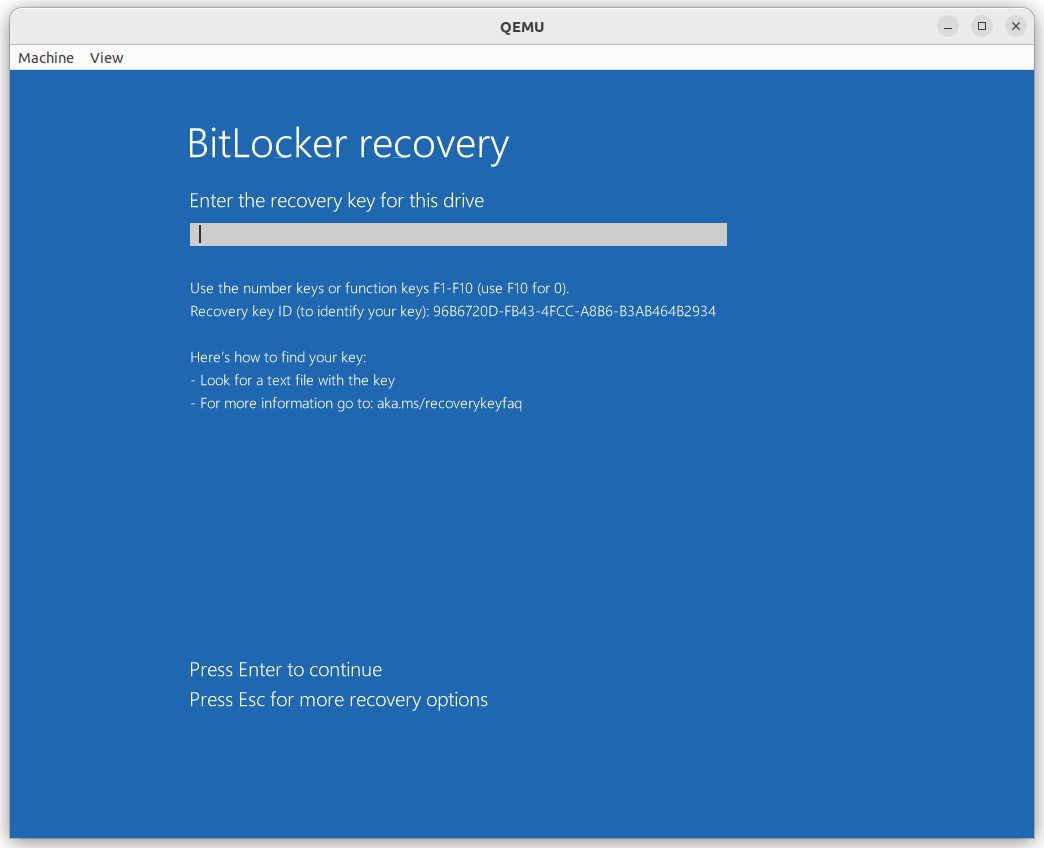
\includegraphics[width=\textwidth]{attacks/bitlocker/01_recovery_prompt.png}

% tpm values different
This happens due to TPM PCR values differing from what was initially used to seal the VMK, leaving the Windows bootloader unable to retrieve an unencrypted VMK from the TPM and as a result unable to decrypt the Windows installation. \TODO{the two different bitlocker volumes}

% bitlocker auto decryption fails
% boot execution differs from executing rootkit
\TODO{which measurements are used for sealing and unsealing}
\TODO{which ones are altered by the rootkit being present}


In theory this is as far as we get, BitLocker in combination of TPM measurements successfully mitigates UEFI attacks by disovering a deviation in the boot flow.
% what is the reaction of the average user
In practice we have to ask ourselves the question how a user reacts to seeing the BitLocker recovery prompt and the consequences to the action the user takes. As an immediate reaction the user has two options: entering the recovery key into the prompt or not entering the recovery key.
% motivation behind user decision
What decision the user makes is dependent on their tech saviness and influenced by a variety of factors such as urgency of booting into Windows, knowing alternatives to what the prompt tells them.
It is reasonable to assume that the average user is willingly entering their recovery key in response to the prompt as the prompt does not suggest any malicious causes or any negative reprocussions in following the instructions. The link mentioned in the prompt also only aids in locating the reocvery key \cite{microsoft-recovery-key-faq}.
\TODO{mention microsofts reasons for the prompt to be triggered}
\TODO{what is the actual alternative}
% does the user trust the system
% why would they not trust the system
% (ask admin for recovery password)
% type in recovery password
% alternative would be to remove drive and insert into safe device

Having the user enter their recovery key does not directly benefit our endevaours as BitLocker does not en/decrypt the hard drive as a whole upon boot but instead performs these respective action when reading or writing a block of data to or from the hard drive.

What we can do is try to record the keystrokes performed by the user while entering their recovery key and use it at some later point to gain control over the hard drive. A program designed to perform this type of attack is called a keylogger.

To implement such a keylogger we have to alter the code execution that happens when the recovery prompt is shown. For this our first step is to find our what execution environment or UEFI stage we are in, is Windows already using separate drivers for keyboard access or still relying on the UEFI environment and its protocols.

% ref to background os loader
% prompt is done by the OS Loader
% ergo still during transient system load phase
% required to use protocol services
% therefor uses uefi services for IO
% such as SimpleTextInputEx Protocol
% go over the two different input protocols
% find out which one is used
The UEFI specification defines two protocols which are used to abstract keyboard input these are the \lstinline{{SimpleTextInputProtocol} and the \lstinline{{SimpleTextInputExProtocol} \cite[12.2, 12.3]{uefi-spec}. To figure out if the recovery prompt uses these to read key strokes we can just add some print statements to the \lstinline{ReadKeyStroke} and \lstinline{ReadKeyStrokeEx} functions of their implementations in the edk2 OVMF package. On the next boot when typing we find that our \lstinline{ReadKeyStrokeEx} print statements from the \lstinline{{SimpleTextInputExProtocol} are triggered.

Now, knowing that the BitLocker recovery prompt is shown by an application running in the UEFI boottime environment, we can leverage this environment to implement our keylogger.

% explain more in depth how protocols are returned to the end user
% one instance per controller/handle
\TODO{how are protocols returned to the end user}
% explain basic back to the caller. This method is called function hooking
% explain how we retain information of the hook in question
% map protocol pointer to hook information
% keylog recovery key
To alter the code execution when performing a key stroke we can just iterate over all instances of the \lstinline{{SimpleTextInputExProtocol} and reassign the \lstinline{ReadKeyStrokeEx} entry of the struct, which is a function pointer. We will save each protocol instances' original function address and instead have it point to an intermediary function. This intermediary calls the original function and performs logging of the key stroke result before relaying the result to the caller. This method is called function hooking and is intransparent to consumer of a protocol.

%  show whole protocol
% WaitForKeyEx event
% wait for event
% query which key it was

\TODO{how is the SimpleTextInputEx Protocol used}

So far we are able to track each keystroke that queried via the \lstinline{ReadKeyStrokeEx} function, which in our testing is only done during the recovery prompt, but may be used by BIOS interactive menu.

\TODO{key input advancment is weird and makes tracking tricky}
F keys
block validity
only divisable by 11
cursor can move out of incomplete or valid blocks
up and down increments or decrements the cursor position

alternatively screen shot
still need hook to find when enter is pressed
explain how screenshotting works
some basic compression
wait for recovery key
send recovery key on enter press

on real hardware
network stack wasn't installed onto handles when boot over ip was disabled
compared loaded dxe drivers between both configurations with efi shell
Realtek Family driver not loaded
load manually
reinstall all handle to controllers to enable network stack regardless

sending key out is only good for physical access attack vector
dislocker linux utility
\cite{dislocker}
mount encrypted drive with decryption mean
read and write access
dual boot in vm
enter recovery key and it works
port to uefi

bitlocker encrypts block-wise

% blk and fs
\TODO{explain block devices}
\TODO{explain file system indepent abstraction better}
uefi protocol stack
\TODO{diagram of block io, disk io, simple filesystem and file protocol interaction (with hindsight of adding dislocker beneath block io)}
\cite[13.3.2 Partition Disocvery]{uefi-spec}
Drivers providing Simple File System Protocol use the Block I/O Protocol to access the underlying media.


hook block io
again hook data mapping

% execute after NTFS driver by doing it in an ExitBootServices hook
It is beneficial for us to write our payload to the Windows installation as close to the end of the UEFI environment as possible, this will maximize the presence of drivers and their offered access to hardware devices. It is also a wise design decision for the attacks following to this one. The call of the function \lstinline{ExitBootServices} marks the point of transitioning from boot time to runtime where the operating system takes over the control of the system, it presents a good opportunity for us to perform the write action of our rootkit.
% was muss man beachten bei exitbootservices hooking
\cite{exitbootservices-hooking}
hook ExitBootServices
enable hook
write payload
import registry key
disable hook

next boot would require to recovery key again
% https://learn.microsoft.com/en-us/windows/security/information-protection/bitlocker/bitlocker-use-bitlocker-drive-encryption-tools-to-manage-bitlocker
update tpm values in payload
caveat pin? look into this

% reference to rootkit definition
persistence when part of root of trust
fresh install / tpm update values
% paper von betreuern
hook Trusted Copmuting Group 2 (TCG2) Protocol
TPM communication
\cite[6.7.3]{tcg-efi-platform-spec}
% \cite[12.7 TPM_Unseal]{tcg-tpm-library-part3-commands}
receive bitlocker vmk key and send to dislocker

% https://labs.withsecure.com/publications/sniff-there-leaks-my-bitlocker-key
% !TeX root = ../thesis.tex

\chapter{Results}
% !TeX root = ../thesis.tex

% https://www.scribbr.com/research-paper/discussion/

% meaning, importance, and relevance of your results
% explaining and evaluating what you found, showing how it relates to your literature review

\chapter{Discussion}


Our attacks show, the differences between \ac{UEFI} firmware rootkits and \ac{UEFI} bootkits.


% bootkit vs rootkit
bootkit much easier
usb stick, from windows
windows installer
if no password present we can disable secure boot
in case of physical presence it may require to change boot order
physical presence with bootable usb stick (defeated by secure boot)
genrally defeated by secure boot where as the rootkit isnt
even if secure boot was implemented for FV images, it could be patched if the validation change starts within the image

barrier of entry is higher
exploit to overwrite spi flash or be delivered with supply chain difficult
physical presence remove spi chip and emulate spi chip or modify chip content
but high payoff with persistence

% persistence
bootkit moves with hard drive but can be overwritten by fresh install
rootkit persistence across reinstallations or hard drive replacements


% SMM rootkit very powerful, complete control over the system
% \cite{}  https://pdfs.semanticscholar.org/68e7/42523f493b78111031a5a221a8cf767064f4.pdf

% attack assumption reflected to real world aplicability
didnt prevent firmware update overwriting our payload
generally the bitlocker reocvery prompt can raise suspicion and may lead to investigations and the threat to be found
BitLogger is more of a last resort and a social engineering aspect comparable to phishing
implications of windows secure boot PCR7 binding and use of secure boot system integrity check and validation profile 7, 11 is a bad decision of microsoft, that for example allows stolen laptops to be unlocked when infecting the firmware with our rootkit

it is generally very easy to attack windows from the \ac{UEFI} environment and there is little that they can do, as especially all windows code can be patched


\section{Mitigations}

bios password against secure boot removal or bootkit installation from USB

windows cant assume what the implementation of ReadKeyStrokeEx looks like (normally function patching might have a jump etc, which we dont even have here)

hardware validated boot to start the validation change from outside the image

inaccessible spi flash

tpm + pin/usb detectability

\subsection{User awareness}

% https://learn.microsoft.com/en-us/windows/security/information-protection/bitlocker/bitlocker-group-policy-settings#configure-the-pre-boot-recovery-message-and-url
% https://learn.microsoft.com/en-us/windows/security/information-protection/bitlocker/bcd-settings-and-bitlocker
you can change recovery message and URL in BCD hive


% https://learn.microsoft.com/en-us/windows/security/information-protection/bitlocker/bitlocker-recovery-guide-plan

recovery guide

what causes bitlocker recovery
- password wrong too often
- TPM 1.2, changing the BIOS or firmware boot device order
- Having the CD or DVD drive before the hard drive in the BIOS boot order and then inserting or removing a CD or DVD
- Failing to boot from a network drive before booting from the hard drive.
- Docking or undocking a portable computer
- Changes to the NTFS partition table on the disk including creating, deleting, or resizing a primary partition.
- Entering the personal identification number (PIN) incorrectly too many times
- Upgrading critical early startup components, such as a BIOS or UEFI firmware upgrade
- Updating option ROM firmware graphics card
- Adding or removing hardware
- REMOVING, INSERTING, OR COMPLETELY DEPLETING THE CHARGE ON A SMART BATTERY ON A PORTABLE COMPUTER
- Pressing the F8 or F10 key during the boot process
what does the recovery screen say \autoref{fig:bitlocker-recovery-prompt}

% https://learn.microsoft.com/en-us/windows/security/information-protection/bitlocker/bitlocker-device-encryption-overview-windows-10
% https://learn.microsoft.com/en-us/mem/configmgr/protect/deploy-use/bitlocker/helpdesk-portal?source=recommendations
% https://learn.microsoft.com/en-us/microsoft-desktop-optimization-pack/mbam-v25/
Enables end users to recover encrypted devices independently by using the Self-Service Portal

googeln wie legitime recovery key prompt reaktion aussieht

enterprise policy recovery key einschraenkbar?

enterprise policy on recovery key loss

vermitteln was das prompt bedeuten koennte

aber kann man einfach nicht anzeigen lassen

Security Flaw of entering a Recovery Password in an inheritly unsafe System

enterprise doesnt hand out recovery keys and instead receives hard drive


!!!!!!!!!!!!!!!!!!!!!!!!!
without hardware chain of trust a compromised system can patch/change any software and fixes are impossible

phishing prompts on their own
% !TeX root = ../thesis.tex

\chapter{Conclusion}
\label{sec:conclusion}

Our practical analysis of \ac{UEFI} threats against Windows 11 showed that enabling Secure Boot when using BitLocker comes with a hidden reduction in security.
Microsoft misuses Secure Boot in an attempt to provide platform firmware integrity validation, where the \ac{TPM} already offers a perfectly fine solution.
With such a misconfigured BitLocker validation profile our rootkit was able to sniff the communication between the Windows Boot Manager and \ac{TPM} without introducing side effects.
Through interception of the \emph{unseal} command, we gained access to the unencrypted BitLocker \ac{VMK}, to decrypt the hard drive and deploy further payload in the Windows installation.
By then modifying the Windows registry our payload was executed with privileges of the local system account.

Microsoft also has set a dangerous precedent by offering the user a mechanism to override the security reaction to integrity violations in an inherently untrustworthy system.
In the case of a correctly configured BitLocker validation profile, the code of our root- or bootkit measured into the \ac{TPM} cause the \emph{unseal} operation to fail and the Windows Boot Manager to trigger a recovery prompt.
The burden of security enforcement is now left to the user and when they decide to put further trust into the system and enter their recovery key, our \emph{BitLogger} can record the performed keystrokes to decrypt the hard drive.

\section*{Future Work}

It would be interesting to take a closer look at memory\-/based attacks under the light of \ac{VBS} like \ac{HVCI} and how rootkits might interact with the \ac{SMM} to circumvent these security mechanisms.
Further investigations into platforms where the \ac{RTM} is being established by the \ac{SRTM} measuring itself, could reveal these implementations to be much more vulnerable against rootkits than laid out in this thesis.
Verifying whether the current implementations of \ac{HVB} provide a gapless security chain might be of similar interest.


% --------------------------
% Back matter
% --------------------------
%
{%
    \setstretch{1.1}
    \renewcommand{\bibfont}{\normalfont\small}
    \setlength{\biblabelsep}{0pt}
    \setlength{\bibitemsep}{0.5\baselineskip plus 0.5\baselineskip}
    \printbibliography[nottype=online]
    \newrefcontext[labelprefix={@}]
    \printbibliography[heading=subbibliography,title={Webpages},type=online]
}
\cleardoublepage

\listoffigures
\cleardoublepage

\listoftables
\cleardoublepage

\lstlistoflistings
\cleardoublepage

\appendix\cleardoublepage
% !TEX root = ../thesis.tex

\chapter{Appendix}

\section{System Table}
\lstinputlisting[language=C,caption={System Table},captionpos=b,label=lst:system-table]{code/system_table.h}
\clearpage

\subsection{Boot Services}
\lstinputlisting[language=C,caption={Boot Services},captionpos=b,label=lst:boot-services]{code/boot_services.h}
\clearpage

\subsection{Runtime Services}
\lstinputlisting[language=C,caption={Runtime Services},captionpos=b,label=lst:runtime-services]{code/runtime_services.h}
\clearpage

\section{Protocols}

\subsection{Loaded Image Protocol}
\lstinputlisting[language=C,firstline=4,caption={Loaded Image Protocol},captionpos=b,label=lst:loaded-image-protocol]{code/protocols/LoadedImage.h}

\clearpage

\subsection{Driver Binding Protocol}
\lstinputlisting[language=C,firstline=4,caption={Driver Binding Protocol},captionpos=b,label=lst:driver-binding-protocol]{code/protocols/DriverBinding.h}

\clearpage

\subsection{Simple File System and File Protocol}
\lstinputlisting[language=C,firstline=4,caption={Simple File System and File Protocol},captionpos=b,label=lst:simple-file-system-protocol]{code/protocols/SimpleFileSystem.h}

\clearpage

\subsection{Disk \acs{I/O} Protocol}
\lstinputlisting[language=C,firstline=4,caption={Disk \ac{I/O} Protocol},captionpos=b,label=lst:disk-io-protocol]{code/protocols/DiskIo.h}

\clearpage

\subsection{Block \acs{I/O} Protocol}
\lstinputlisting[language=C,firstline=4,caption={Block \ac{I/O} Protocol},captionpos=b,label=lst:block-io-protocol]{code/protocols/BlockIo.h}

\clearpage

\subsection{\acf{BDS} Protocol}

\lstinputlisting[language=C,firstline=4,caption={\ac{BDS} Protocol},captionpos=b,label=lst:tcg2-protocol]{code/protocols/Bds.h}

\clearpage

\subsection{Firmware Volume2 Protocol}

\lstinputlisting[language=C,firstline=4,caption={\ac{BDS} Protocol},captionpos=b,label=lst:firmware-volume2-protocol]{code/protocols/FirmwareVolume2.h}

\clearpage

\subsection{Simple Text Input Protocol}
\lstinputlisting[language=C,firstline=4,caption={Simple Text Input Ex Protocol},captionpos=b,label=lst:simple-text-input-protocol]{code/protocols/SimpleTextIn.h}

\clearpage

\subsection{Simple Text Input Ex Protocol}
\lstinputlisting[language=C,firstline=4,caption={Simple Text Input Ex Protocol},captionpos=b,label=lst:simple-text-input-ex-protocol]{code/protocols/SimpleTextInEx.h}

\clearpage

\subsection{\acs{TCG}2 Protocol}
\lstinputlisting[language=C,firstline=4,caption={\ac{TCG}2 Protocol},captionpos=b,label=lst:tcg2-protocol]{code/protocols/Tcg2Protocol.h}

\clearpage


\section{Firmware File Types}

\begin{table}[htb]
    \label{tab:file-types}
    \centering
    \small
    \begin{tabularx}{1.05\textwidth}{XcX}
        \toprule
        \textbf{Name}                                                                  & \textbf{Value}          & \textbf{Description}                                                                                                        \\
        \midrule
        \code{EFI\_FV\_FILETYPE\_RAW}                                                  & \code{0x01}             & Binary data                                                                                                                 \\
        \arrayrulecolor{gray}
        \midrule[0.3pt]
        \code{EFI\_FV\_FILETYPE\_FREEFORM}                                             & \code{0x02}             & Sectioned data                                                                                                              \\
        \midrule[0.3pt]
        \code{EFI\_FV\_FILETYPE\_SECURITY\_CORE}                                       & \code{0x03}             & Platform core code used during the SEC phase                                                                                \\
        \midrule[0.3pt]
        \code{EFI\_FV\_FILETYPE\_PEI\_CORE}                                            & \code{0x04}             & PEI Foundation                                                                                                              \\
        \midrule[0.3pt]
        \code{EFI\_FV\_FILETYPE\_DXE\_CORE}                                            & \code{0x05}             & DXE Foundation                                                                                                              \\
        \midrule[0.3pt]
        \code{EFI\_FV\_FILETYPE\_PEIM}                                                 & \code{0x06}             & PEI module (PEIM)                                                                                                           \\
        \midrule[0.3pt]
        \code{EFI\_FV\_FILETYPE\_DRIVER}                                               & \code{0x07}             & DXE driver                                                                                                                  \\
        \midrule[0.3pt]
        \code{EFI\_FV\_FILETYPE\_COMBINED\_PEIM\_DRIVER}                               & \code{0x08}             & Combined PEIM/DXE driver                                                                                                    \\
        \midrule[0.3pt]
        \code{EFI\_FV\_FILETYPE\_APPLICATION}                                          & \code{0x09}             & Application                                                                                                                 \\
        \midrule[0.3pt]
        \code{EFI\_FV\_FILETYPE\_MM}                                                   & \code{0x0A}             & Contains a PE32+ image that will be loaded into MMRAM in MM Traditional Mode.                                               \\
        \midrule[0.3pt]
        \code{EFI\_FV\_FILETYPE\_FIRMWARE\_VOLUME\_IMAGE}                              & \code{0x0B}             & Firmware volume image                                                                                                       \\
        \midrule[0.3pt]
        \code{EFI\_FV\_FILETYPE\_COMBINED\_MM\_DXE}                                    & \code{0x0C}             & Contains PE32+ image that will be dispatched by the DXE Dispatcher and will also be loaded into MMRAM in MM Tradition Mode. \\
        \midrule[0.3pt]
        \code{EFI\_FV\_FILETYPE\_MM\_CORE}                                             & \code{0x0D}             & MM Foundation that support MM Traditional Mode.                                                                             \\
        \midrule[0.3pt]
        \code{EFI\_FV\_FILETYPE\_MM\_STANDALONE}                                       & \code{0x0E}             & Contains a PE32+ image that will be loaded into MMRAM in MM Standalone Mode.                                                \\
        \midrule[0.3pt]
        \code{EFI\_FV\_FILETYPE\_MM\_CORE\_STANDALONE}                                 & \code{0x0F}             & MM Foundation that support MM Tradition Mode and MM Standalone Mode.                                                        \\
        \midrule[0.3pt]
        \code{EFI\_FV\_FILETYPE\_OEM\_MIN\dots} \code{EFI\_FV\_FILETYPE\_OEM\_MAX}     & \code{0xC0}-\code{0xDF} & OEM File Types                                                                                                              \\
        \midrule[0.3pt]
        \code{EFI\_FV\_FILETYPE\_DEBUG\_MIN\dots} \code{EFI\_FV\_FILETYPE\_DEBUG\_MAX} & \code{0xE0}-\code{0xEF} & Debug/Test File Types                                                                                                       \\
        \midrule[0.3pt]
        \code{EFI\_FV\_FILETYPE\_FFS\_MIN\dots} \code{EFI\_FV\_FILETYPE\_FFS\_MAX}     & \code{0xF0}-\code{0xFF} & Firmware File System Specific File Types                                                                                    \\
        \midrule[0.3pt]
        \code{EFI\_FV\_FILETYPE\_FFS\_PAD}                                             & \code{0xF0}             & Pad File For FFS                                                                                                            \\
        \arrayrulecolor{black}
        \bottomrule
    \end{tabularx}
    \caption{Firmware File Types \cite[Vol. 3, Table 3-3]{pi-spec}}

    \normalsize
\end{table}

\clearpage

\section{Firmware File Section Types}

\begin{table}[htb]
    \label{tab:file-section-types}
    \centering
    \small
    \begin{tabularx}{1.0\textwidth}{XcX}
        \toprule
        \textbf{Name}                               & \textbf{Value} & \textbf{Description}                                                                                                                                    \\
        \midrule
        \code{EFI\_SECTION\_COMPRESSION}            & \code{0x01}    & Encapsulation section where other sections are compressed.                                                                                              \\
        \arrayrulecolor{gray}
        \midrule[0.3pt]
        \code{EFI\_SECTION\_GUID\_DEFINED}          & \code{0x02}    & Encapsulation section where other sections have format defined by a \acs{GUID}.                                                                         \\
        \midrule[0.3pt]
        \code{EFI\_SECTION\_DISPOSABLE}             & \code{0x03}    & Encapsulation section used during the build process but not required for execution.                                                                     \\
        \midrule[0.3pt]
        \code{EFI\_SECTION\_PE32}                   & \code{0x10}    & PE32+ Executable image.                                                                                                                                 \\
        \midrule[0.3pt]
        \code{EFI\_SECTION\_PIC}                    & \code{0x11}    & Position-Independent Code.                                                                                                                              \\
        \midrule[0.3pt]
        \code{EFI\_SECTION\_TE}                     & \code{0x12}    & Terse Executable image.                                                                                                                                 \\
        \midrule[0.3pt]
        \code{EFI\_SECTION\_DXE\_DEPEX}             & \code{0x13}    & DXE Dependency Expression.                                                                                                                              \\
        \midrule[0.3pt]
        \code{EFI\_SECTION\_VERSION}                & \code{0x14}    & Version, Text and Numeric.                                                                                                                              \\
        \midrule[0.3pt]
        \code{EFI\_SECTION\_USER\_INTERFACE}        & \code{0x15}    & User-Friendly name of the driver.                                                                                                                       \\
        \midrule[0.3pt]
        \code{EFI\_SECTION\_COMPATIBILITY16}        & \code{0x16}    & DOS-style 16-bit EXE.                                                                                                                                   \\
        \midrule[0.3pt]
        \code{EFI\_SECTION\_FIRMWARE\_VOLUME\_IMAG} & \code{0x17}    & PI Firmware Volume image.                                                                                                                               \\
        \midrule[0.3pt]
        \code{EFI\_SECTION\_FREEFORM\_SUBTYPE\_GUI} & \code{0x18}    & Raw data with GUID in header to define format.                                                                                                          \\
        \midrule[0.3pt]
        \code{EFI\_SECTION\_RAW}                    & \code{0x19}    & Raw data.                                                                                                                                               \\
        \midrule[0.3pt]
        \code{EFI\_SECTION\_PEI\_DEPEX}             & \code{0x1B}    & PEI Dependency Expression.                                                                                                                              \\
        \midrule[0.3pt]
        \code{EFI\_SECTION\_MM\_DEPEX}              & \code{0x1C}    & Leaf section type for determining the dispatch order for an MM Traditional driver in MM Traditional Mode or MM Standalone driver in MM Standalone Mode. \\
        \arrayrulecolor{black}
        \bottomrule
    \end{tabularx}
    \caption{Firmware File Section Types \cite[Vol. 3, Table 3-4]{pi-spec}}
    \normalsize
\end{table}
       % INCLUDE: appendix

\cleardoublepage
% !TEX root = ../thesis.tex

\chapter*{List of Acronyms}
\label{sec:acronyms}

\begin{acronym}[DEPEX]
    \acro{ACPI}{Advanced Configuration and Power Interface}%
    \acro{AES}{Advanced Encryption Standard}%
    \acro{AL}{Afterlife}%
    \acro{API}{Application Programming Interface}%
    \acro{ASCII}{American Standard Code for Information Interchange}%
    \acro{BCD}{Boot Configuration Data}%
    \acro{BDE}{BitLocker Drive Encryption}%
    \acro{BDS}{Boot Device Selection}%
    \acro{BF}{Boot Firmware}%
    \acro{BFV}{\acl{BF} Volume}%
    \acro{BIOS}{Basic \acl{I/O} System}%
    \acro{CA}{Certificate Authority}%
    \acro{CAR}{Cache as \acl{RAM}}%
    \acro{CD}{Compact Disc}%
    \acro{CRTM}{Core \acl{RTM}}%
    \acro{CSM}{Compatibility Support Module}%
    \acro{CPU}{Central Processing Unit}%
    \acro{DB}{Data Base}%
    \acro{DEPEX}{Dependency Expression}%
    \acro{DLL}{Dynamically Linked Library}%
    \acro{DXE}{Driver Execution Environment}%
    \acro{EDK}{\acs{EFI} Development Kit}%
    \acro{EFI}{Extensible Firmware Interface}%
    \acro{ELAM}{Early-Launch Antimalware}%
    \acro{ESP}{\acs{EFI} System Partition}%
    \acro{FAT}{File Allocation Table}%
    \acro{FD}{Firmware Device}%
    \acro{FDF}{Flash Description File}%
    \acro{FFS}{Firmware Filesystem}%
    \acro{FUSE}{Filesystem in Userspace}%
    \acro{FV}{Firmware Volume}%
    \acro{FVE}{Full Volume Encryption}%
    \acro{FVEK}{\acl{FVE} Key}%
    \acro{GPT}{\acs{GUID} Partition Table}%
    \acro{GUID}{Globally Unique Identifier}%
    \acro{HOB}{Hand-off Block}%
    \acro{H-CRTM}{Hardware-\acl{CRTM}}%
    \acro{I/O}{Input/Output}%
    \acro{IBB}{Initial Boot Block}%
    \acro{KEK}{Key Exchange Key}%
    \acro{LBA}{Logical Block Address}%
    \acro{LPC}{Low Pin Count}%
    \acro{MBR}{Master Boot Record}%
    \acro{NTFS}{New Technology File System}%
    \acro{NVRAM}{Non\-/volatile \acs{RAM}}%
    \acro{OEM}{Original Equipment Manufacturer}%
    \acro{OS}{Operating System}%
    \acro{OVMF}{Open Virtual Machine Firmware}%
    \acro{PC}{Personal Computer}%
    \acro{PCI}{Peripheral Component Interconnect}%
    \acro{PCR}{Platform Configuration Register}%
    \acro{PE32}{Portable Executable 32-Bit}%
    \acro{PEI}{Pre-\acs{EFI} Initialization}%
    \acro{PEIM}{\acl{PEI} Module}%
    \acro{PF}{Platform Firmware}%
    \acro{PI}{Platform Initialization}%
    \acro{PIN}{Personal Identification Number}%
    \acro{PK}{Platform Key}%
    \acro{PPI}{\acs{PEIM}-to-\acs{PEIM} Interface}%
    \acro{QEMU}{Quick Emulator}%
    \acro{RAM}{Random Access Memory}%
    \acro{ROM}{Read-Only Memory}%
    \acro{RT}{Runtime}%
    \acro{RTM}{Root of Trust for Measurement}%
    \acro{RTM}{Root of Trust for Storage}%
    \acro{SEC}{Security}%
    \acro{SMM}{System Management Mode}%
    \acro{SRTM}{Static Root of Trust for Measurement}%
    \acro{SPI}{Serial Peripheral Interface}%
    \acro{TB}{Terra Byte}%
    \acro{TCG}{Trusted Computing Group}%
    \acro{TPM}{Trusted Platform Module}%
    \acro{TSL}{Transient System Load}%
    \acro{UEFI}{Unified \acl{EFI}}%
    \acro{USB}{Universal Serial Bus}%
    \acro{UUID}{Universally Unique Identifier}%
    \acro{VBR}{Volume Boot Record}%
    \acro{VMK}{Volume Master Key}%
    \acro{XML}{Extensible Markup Language}%
\end{acronym}
\clearpage

\newpage
\mbox{}

\end{document}